\documentclass[a4paper, 12pt]{article}
\usepackage[a4paper,top=1.5cm, bottom=1.5cm, left=1cm, right=1cm]{geometry}

% Работа с русским языком
\usepackage[utf8]{inputenc}
\usepackage{mathtext}                % русские буквы в формулах
\usepackage[english, russian]{babel} % локализация и переносы

\usepackage{graphicx}   % Вставка изображений
\usepackage{float}      % "Плавающие" изображения3
\usepackage{wrapfig}    % Обтекание фигур (таблиц, картинок и прочего)
\graphicspath{ {./images/} }

\usepackage{tabularx}
\usepackage{multirow}
\usepackage{amsmath}
\usepackage{amsfonts}
\usepackage{indentfirst}
\usepackage{longtable}
\graphicspath{{pictures/}}
\usepackage{natbib}

%%% Колонтитулы
\usepackage{titleps}
\newpagestyle{main}{
	\setheadrule{0.4pt}
	\sethead{Отчёт о выполнении лабораторной работы 2.2.3}{}{}
	\setfootrule{0.4pt}                       
	\setfoot{ФРКТ МФТИ, 2023}{}{\thepage} 
}
\pagestyle{main}  

\begin{document}
    \begin{titlepage}
	\begin{center}
            {\large МОСКОВСКИЙ ФИЗИКО-ТЕХНИЧЕСКИЙ ИНСТИТУТ (НАЦИОНАЛЬНЫЙ       ИССЛЕДОВАТЕЛЬСКИЙ УНИВЕРСИТЕТ)}
	\end{center}
 
	\begin{center}
		{\large Физтех-школа радиотехники и компьютерных технологий}
	\end{center}
	
	\vspace{8cm}
	{\LARGE
		\begin{center}
                {\bf Отчёт о выполнении лабораторной работы 2.2.3}\\
                Измерение теплопроводности воздуха при атмосферном давлении
		\end{center}
	}
	\vspace{5cm}
	\begin{flushright}
		{\Large Автор:\\ Тихонов Дмитрий Романович, \\
			\vspace{0.2cm}
			студент группы Б01-206}
	\end{flushright}
	\vspace{5cm}
	\begin{center}
		\Large Долгопрудный, 2023
	\end{center}
    \end{titlepage}

    \section*{Введение}
        \noindent \textbf{Цель работы:} измерить коэффициент теплопроводности воздуха при атмосферном давлении в зависимости от температуры.\\
        
        \noindent \textbf{В работе используются:} цилиндрическая колба с натянутой по оси нитью; термостат; вольтметр и амперметр (цифровые мультиметры); эталонное сопротивление; источник постоянного напряжения; магазин сопротивлений.

    \section*{Теоретические сведения}
        \noindent \textit{Теплопроводность} - это процесс передачи тепловой энергии от нагретых частей системы к холодным за счёт хаотического движения частиц среды (молекул, атомов и т.п.). В газах теплопроводность осуществляется за счёт непосредственной передачи кинетической энергии от быстрых молекул к медленным при их столкновениях. Перенос тепла описывается \textit{законом Фурье}.
    
    \begin{equation}
        \overrightarrow{q}=-\kappa\cdot \nabla T
    \end{equation}

    \noindent где $\overrightarrow{q} \: [\frac{\text{Вт}}{\text{м}^2}]$ - плотность потока энергии, $\kappa \sim \lambda\bar{\upsilon}\cdot n c_v$ - коэффициент теплопроводности.\\

    \noindent Длина свободного пробега может быть оценена как $\lambda = 1/n \sigma$, где $\sigma$ — эффективное сечение столкновений молекул друг с другом. Отсюда, коэффициент теплопроводности газа не зависит от плотности газа и определяется только его температурой. В простейшей модели твёрдых шариков $\sigma = const$, и коэффициент теплопроводности пропорционален корню абсолютной температуры: $\kappa \propto \bar{\upsilon} / \sigma \propto \sqrt{T}$. На практике эффективное сечение $\sigma(T)$ следует считать медленно убывающей функцией $T$.\\
    
    \noindent Рассмотрим стационарную теплопроводность в цилиндрической геометрии (рис. \ref{Цилиндр}). Если цилиндр длинный ($L \gg r_0$), можно пренебречь теплоотводом через его торцы. Тогда все параметры газа можно считать зависящими только от расстояния до оси системы $r$ а поток тепла $\overrightarrow{q}$ направленным строго радиально. Для стационарного режима и малого перепада температуры между нитью и стенками цилиндра:
    
    \begin{equation}
        Q = -2\pi r L\cdot \kappa \frac{dT}{dr}=\frac{2\pi L}{ln\frac{r_0}{r_1}}\kappa\cdot \Delta T
        \label{formula}
    \end{equation}

    \begin{figure}[H]
        \centering
        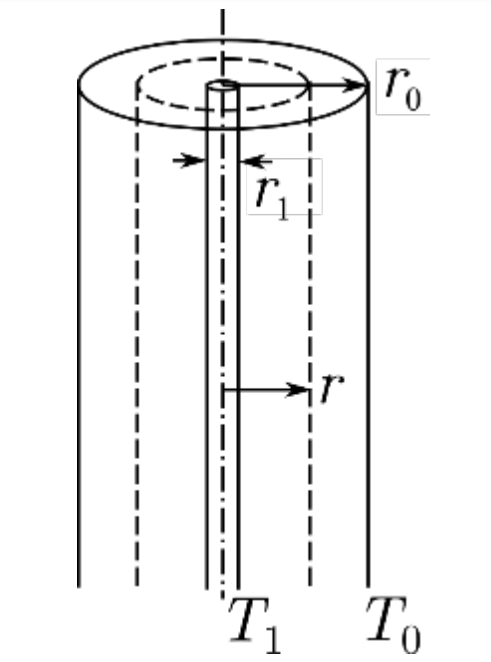
\includegraphics[width=0.3\textwidth]{images/cylinder.png}
        \caption{Геометрия измерений} 
        \label{Цилиндр}
    \end{figure}

    \section*{Методика измерений и используемое оборудование}
    
        \noindent Схема установки представлена на рис. \ref{Схема установки}. Полость трубки заполнена воздухом (полость через небольшое отверстие сообщается с атмосферой). Стенки трубки помещены в кожух, через которых пропускается вода из термостата, так что их температура поддерживается постоянной. Для предотвращения конвекции трубка расположена вертикально. Металлическая нить служит как источником тепла, так и датчиком температуры (термометром сопротивления).

        \begin{figure}[H]
            \centering
            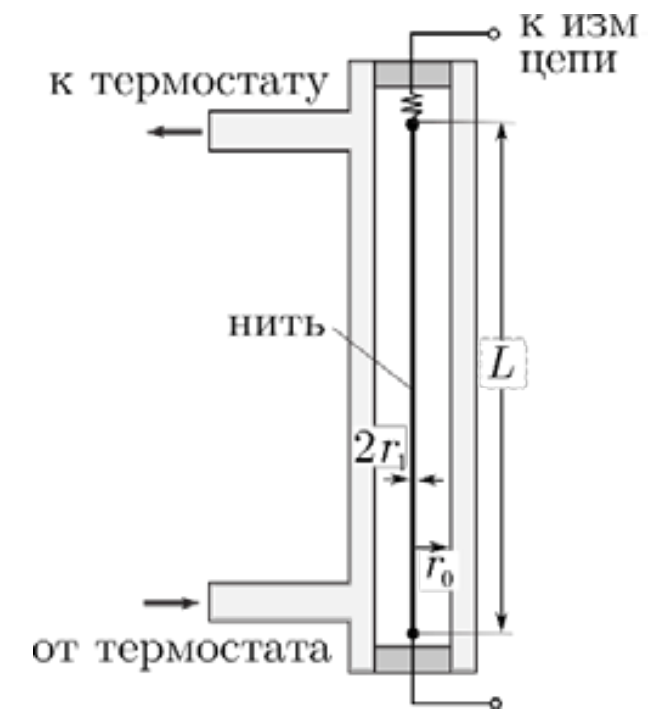
\includegraphics[width=0.3\textwidth]{images/tube.png}
            \caption{Схема установки} 
            \label{Схема установки}
        \end{figure}

        \noindent Для большинства металлов изменение сопротивления из-за нагрева невелико: при изменении температуры на $\Delta t = 1 ^\circ C$ относительное изменение сопротивления нити может составлять приблизительно от 0.5\% (в зависимости от её материала). Следовательно, измерение важно провести с высокой точностью.\\
        
        \noindent Электрическая схема установки на рис. \ref{ЭлектрическаяСхема}.  Для измерения напряжения и тока используется два мультиметра, работающие в режимах вольтметра и амперметра соответственно. По двум проводам (токовая пара $I_+$ и $I_-$) через сопротивление пропускается измерительный ток, а два других (потенциальная пара $U_+$ и $U_-$) используются для параллельного подключения вольтметра. Заметим, что при такой схеме внутреннее сопротивление приборов и сопротивление подводящих проводов практически не влияет на измерения: сопротивление амперметра не влияет на результат вовсе, а сопротивление вольтметра составляет обычно 1–100 МОм, что при $R_\text{н} = 20 \text{ Ом}$ вносит относительную ошибку не более $10^{-5}$.

        \begin{figure}[H]
            \centering
            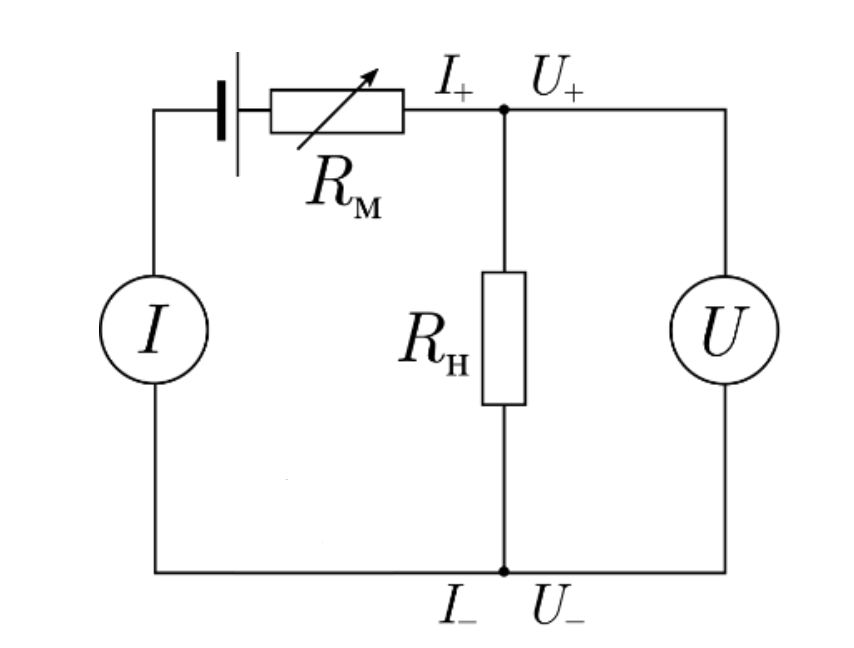
\includegraphics[width=0.5\textwidth]{images/circuit.png}
            \caption{Электрическая схема установки} 
            \label{ЭлектрическаяСхема}
        \end{figure}

        \noindent Ток цепи регулируется с помощью магазина сопротивлений, включенного последовательно с источником напряжения. Измерение нагрузочных кривых позволяет получить температурную зависимость сопротивления нити (при $Q \to 0$, $T\approx T_0$). Для исследуемых температур:
        
        \begin{equation}
            R(t)=R_{273}\cdot(1+\alpha t)
        \end{equation}
        
        \noindent $\alpha=\frac{1}{R_{273}}\frac{dR}{dT}$  - температурный коэффициент сопротивления материала.

    \section*{Результаты измерений и обработка данных}
    
        \subsection*{Исследование зависимости $R(Q)$ при разных температурах}
        
        \noindent Снимем зависимость сопротивления нити от мощности $R(Q)$ для каждой из температур (табл. \ref{Данные}). Значения $U$ и $I$ будем снимать, когда установится стационарный режим. Вычислим значения погрешности для $R$ и $Q$ и также занесём эти данные в таблицу \ref{Данные}.

        \begin{table}[H]
            \centering
            \begin{tabular}{|cccccccccc|}
                \hline
                \multicolumn{1}{|c|}{$T$, $^\circ$C} & \multicolumn{9}{c|}{22,0} \\ \hline
                \multicolumn{1}{|c|}{$U$, мВ} & \multicolumn{1}{c|}{38,455}  & \multicolumn{1}{c|}{146,280}  & \multicolumn{1}{c|}{487,180}  & \multicolumn{1}{c|}{733,050} & \multicolumn{1}{c|}{1171,360} & \multicolumn{1}{c|}{1310,640} & \multicolumn{1}{c|}{1800,870} & \multicolumn{1}{c|}{2073,620} & \multicolumn{1}{c|}{2160,230} \\ \hline
                \multicolumn{1}{|c|}{$I$, мА} & \multicolumn{1}{c|}{1,916}   & \multicolumn{1}{c|}{7,289} & \multicolumn{1}{c|}{24,199}   & \multicolumn{1}{c|}{36,266} & \multicolumn{1}{c|}{57,320}   & \multicolumn{1}{c|}{63,870} & \multicolumn{1}{c|}{86,111}   & \multicolumn{1}{c|}{97,978} & \multicolumn{1}{c|}{101,672} \\ \hline
                \multicolumn{1}{|c|}{$Q$, мВт} & \multicolumn{1}{c|}{0,074} & \multicolumn{1}{c|}{1,066} & \multicolumn{1}{c|}{11,789} & \multicolumn{1}{c|}{26,585} & \multicolumn{1}{c|}{67,142} & \multicolumn{1}{c|}{83,711} & \multicolumn{1}{c|}{155,074} & \multicolumn{1}{c|}{203,170} & \multicolumn{1}{c|}{219,634} \\ \hline
                \multicolumn{1}{|c|}{$R$, Ом} & \multicolumn{1}{c|}{20,072}  & \multicolumn{1}{c|}{20,069}   & \multicolumn{1}{c|}{20,133}   & \multicolumn{1}{c|}{20,213}   & \multicolumn{1}{c|}{20,435}   & \multicolumn{1}{c|}{20,520}   & \multicolumn{1}{c|}{20,913}   & \multicolumn{1}{c|}{21,164} & \multicolumn{1}{c|}{21,247} \\ \hline
                \multicolumn{10}{|c|}{} \\ \hline
                \multicolumn{1}{|c|}{$T$, $^\circ$C} & \multicolumn{9}{c|}{32,0} \\ \hline
                \multicolumn{1}{|c|}{$U$, мВ} & \multicolumn{1}{c|}{751,689} & \multicolumn{1}{c|}{1123,100} & \multicolumn{1}{c|}{1349,500} & \multicolumn{1}{c|}{1526,300} & \multicolumn{1}{c|}{1672,720} & \multicolumn{1}{c|}{1803,750} & \multicolumn{1}{c|}{1917,810} & \multicolumn{1}{c|}{2031,250} & \multicolumn{1}{c|}{2119,400} \\ \hline
                \multicolumn{1}{|c|}{$I$, мА} & \multicolumn{1}{c|}{35,931}  & \multicolumn{1}{c|}{53,248}   & \multicolumn{1}{c|}{63,561}   & \multicolumn{1}{c|}{71,464}   & \multicolumn{1}{c|}{77,901}   & \multicolumn{1}{c|}{83,599}   & \multicolumn{1}{c|}{88,471}   & \multicolumn{1}{c|}{93,256} & \multicolumn{1}{c|}{96,966}   \\ \hline
                \multicolumn{1}{|c|}{$Q$, мВт} & \multicolumn{1}{c|}{27,009}  & \multicolumn{1}{c|}{59,803}   & \multicolumn{1}{c|}{85,776}   & \multicolumn{1}{c|}{109,075}  & \multicolumn{1}{c|}{130,307}  & \multicolumn{1}{c|}{150,792}  & \multicolumn{1}{c|}{169,671}  & \multicolumn{1}{c|}{189,426} & \multicolumn{1}{c|}{205,510}  \\ \hline
                \multicolumn{1}{|c|}{$R$, Ом} & \multicolumn{1}{c|}{20,920}  & \multicolumn{1}{c|}{21,092}   & \multicolumn{1}{c|}{21,232} & \multicolumn{1}{c|}{21,358}   & \multicolumn{1}{c|}{21,472} & \multicolumn{1}{c|}{21,576}   & \multicolumn{1}{c|}{21,677}   & \multicolumn{1}{c|}{21,781} & \multicolumn{1}{c|}{21,857}   \\ \hline
                \multicolumn{10}{|c|}{} \\ \hline
                \multicolumn{1}{|c|}{$T$, $^\circ$C} & \multicolumn{9}{c|}{47,0} \\ \hline
                \multicolumn{1}{|c|}{$U$, мВ} & \multicolumn{1}{c|}{833,158} & \multicolumn{1}{c|}{1155,590} & \multicolumn{1}{c|}{1382,310} & \multicolumn{1}{c|}{1558,280} & \multicolumn{1}{c|}{1707,970} & \multicolumn{1}{c|}{1832,120} & \multicolumn{1}{c|}{1943,720} & \multicolumn{1}{c|}{2047,740} & \multicolumn{1}{c|}{2140,610} \\ \hline
                \multicolumn{1}{|c|}{$I$, мА} & \multicolumn{1}{c|}{37,871} & \multicolumn{1}{c|}{52,179} & \multicolumn{1}{c|}{62,055} & \multicolumn{1}{c|}{69,595} & \multicolumn{1}{c|}{75,915} & \multicolumn{1}{c|}{81,096} & \multicolumn{1}{c|}{85,683} & \multicolumn{1}{c|}{89,932} & \multicolumn{1}{c|}{93,674}   \\ \hline
                \multicolumn{1}{|c|}{$Q$, мВт} & \multicolumn{1}{c|}{31,553} & \multicolumn{1}{c|}{60,298} & \multicolumn{1}{c|}{85,779} & \multicolumn{1}{c|}{108,448} & \multicolumn{1}{c|}{129,660} & \multicolumn{1}{c|}{148,577} & \multicolumn{1}{c|}{166,545} & \multicolumn{1}{c|}{184,158} & \multicolumn{1}{c|}{200,520} \\ \hline
                \multicolumn{1}{|c|}{$R$, Ом} & \multicolumn{1}{c|}{22,000} & \multicolumn{1}{c|}{22,147} & \multicolumn{1}{c|}{22,276} & \multicolumn{1}{c|}{22,391} & \multicolumn{1}{c|}{22,499} & \multicolumn{1}{c|}{22,592} & \multicolumn{1}{c|}{22,685} & \multicolumn{1}{c|}{22,770} & \multicolumn{1}{c|}{22,852}   \\ \hline
                \multicolumn{10}{|c|}{} \\ \hline
                \multicolumn{1}{|c|}{$T$, $^\circ$C} & \multicolumn{9}{c|}{62,0} \\ \hline
                \multicolumn{1}{|c|}{$U$, мВ} & \multicolumn{1}{c|}{860,674} & \multicolumn{1}{c|}{1186,705} & \multicolumn{1}{c|}{1413,710} & \multicolumn{1}{c|}{1588,620} & \multicolumn{1}{c|}{1736,640} & \multicolumn{1}{c|}{1858,290} & \multicolumn{1}{c|}{1968,140} & \multicolumn{1}{c|}{2069,940} & \multicolumn{1}{c|}{2160,340} \\ \hline
                \multicolumn{1}{|c|}{$I$, мА} & \multicolumn{1}{c|}{37,323} & \multicolumn{1}{c|}{51,151}   & \multicolumn{1}{c|}{60,607} & \multicolumn{1}{c|}{67,792}   & \multicolumn{1}{c|}{73,804} & \multicolumn{1}{c|}{78,686}   & \multicolumn{1}{c|}{83,050} & \multicolumn{1}{c|}{87,051}   & \multicolumn{1}{c|}{90,572}   \\ \hline
                \multicolumn{1}{|c|}{$Q$, мВт} & \multicolumn{1}{c|}{32,123} & \multicolumn{1}{c|}{60,701}   & \multicolumn{1}{c|}{85,681} & \multicolumn{1}{c|}{107,695}  & \multicolumn{1}{c|}{128,171} & \multicolumn{1}{c|}{146,222}  & \multicolumn{1}{c|}{163,454} & \multicolumn{1}{c|}{180,190}  & \multicolumn{1}{c|}{195,666}  \\ \hline
                \multicolumn{1}{|c|}{$R$, Ом} & \multicolumn{1}{c|}{23,060} & \multicolumn{1}{c|}{23,200} & \multicolumn{1}{c|}{23,326} & \multicolumn{1}{c|}{23,434} & \multicolumn{1}{c|}{23,530} & \multicolumn{1}{c|}{23,616} & \multicolumn{1}{c|}{23,698} & \multicolumn{1}{c|}{23,779} & \multicolumn{1}{c|}{23,852} \\ \hline
                \multicolumn{10}{|c|}{} \\ \hline
                \multicolumn{1}{|c|}{$T$, $^\circ$C} & \multicolumn{9}{c|}{77,0} \\ \hline
                \multicolumn{1}{|c|}{$U$, мВ} & \multicolumn{1}{c|}{314,325} & \multicolumn{1}{c|}{887,557} & \multicolumn{1}{c|}{1216,960} & \multicolumn{1}{c|}{1444,170} & \multicolumn{1}{c|}{1617,700} & \multicolumn{1}{c|}{1763,970} & \multicolumn{1}{c|}{} & \multicolumn{1}{c|}{} & \multicolumn{1}{c|}{} \\ \hline
                \multicolumn{1}{|c|}{$I$, мА} & \multicolumn{1}{c|}{13,102} & \multicolumn{1}{c|}{36,792} & \multicolumn{1}{c|}{50,163} & \multicolumn{1}{c|}{59,239} & \multicolumn{1}{c|}{66,103} & \multicolumn{1}{c|}{71,805} & \multicolumn{1}{c|}{} & \multicolumn{1}{c|}{} & \multicolumn{1}{c|}{} \\ \hline
                \multicolumn{1}{|c|}{$Q$, мВт} & \multicolumn{1}{c|}{4,118} & \multicolumn{1}{c|}{32,655} & \multicolumn{1}{c|}{61,046} & \multicolumn{1}{c|}{85,551} & \multicolumn{1}{c|}{106,935} & \multicolumn{1}{c|}{126,662} & \multicolumn{1}{c|}{} & \multicolumn{1}{c|}{} & \multicolumn{1}{c|}{} \\ \hline
                \multicolumn{1}{|c|}{$R$, Ом} & \multicolumn{1}{c|}{23,990} & \multicolumn{1}{c|}{24,124} & \multicolumn{1}{c|}{24,260} & \multicolumn{1}{c|}{24,379} & \multicolumn{1}{c|}{24,472} & \multicolumn{1}{c|}{24,566} & \multicolumn{1}{c|}{} & \multicolumn{1}{c|}{} & \multicolumn{1}{c|}{} \\ \hline
            \end{tabular}
            \caption{Результаты измерений $U$ и $I$ и результаты вычислений $R$ и $Q$ при разных температурах}
            \label{Данные}
        \end{table}

        \noindent Приведем расчётные формулы для значений $R$ и $Q$:
        \begin{equation}
            R_{\text{н}} = \frac{U}{I}
        \end{equation}

         \begin{equation}
            Q = UI
        \end{equation}

        \noindent Отсюда, находим погрешность вычисления этих величин:
        \begin{equation}
            \sigma_{R_{\text{н}}} = R_{\text{н}} \cdot \sqrt{\left ( \frac{\Delta U}{U}\right)^2 + \left ( \frac{\Delta I}{I}\right)^2} \approx 10^{-2} \text{ мОм}
        \end{equation}

        \begin{equation}
            \sigma_{Q} = Q \cdot \sqrt{\left ( \frac{\Delta U}{U}\right)^2 + \left ( \frac{\Delta I}{I}\right)^2} \approx 10^{-2} \text{ мВт}
        \end{equation}
        \noindent где $\Delta I = 10^{-2} \text{ мА}$, $\Delta U = 10^{-2} \text{ мВ}$ (\textit{данные взяты из технических параметров установки}). Заметим, что в масштабе графика $R_{\text{н}}(Q)$ кресты погрешностей нанести не получится. \\

        \noindent Для каждой температуры прибора построим график зависимости сопротивления нити $R$ от выделяемой мощности $Q$. Аппроксимацию прямой произведем методом наименьших квадратов в компьютерной программе \textit{Origin Pro 2023}, в которой определим наклон $dR/dQ$ с погрешностью и сопротивление нити $R|_{Q = 0}$ при температуре термостата, то есть при нулевой выделяемой мощности. Полученные данные занесём в таблицу~\ref{table:results_2}. Графики представлены на рис.~\ref{graph:R(Q)_22}, рис.~\ref{graph:R(Q)_32}, рис.~\ref{graph:R(Q)_47}, рис.~\ref{graph:R(Q)_62}, рис.~\ref{graph:R(Q)_77}. 

        \begin{figure}[H]
            \centering
            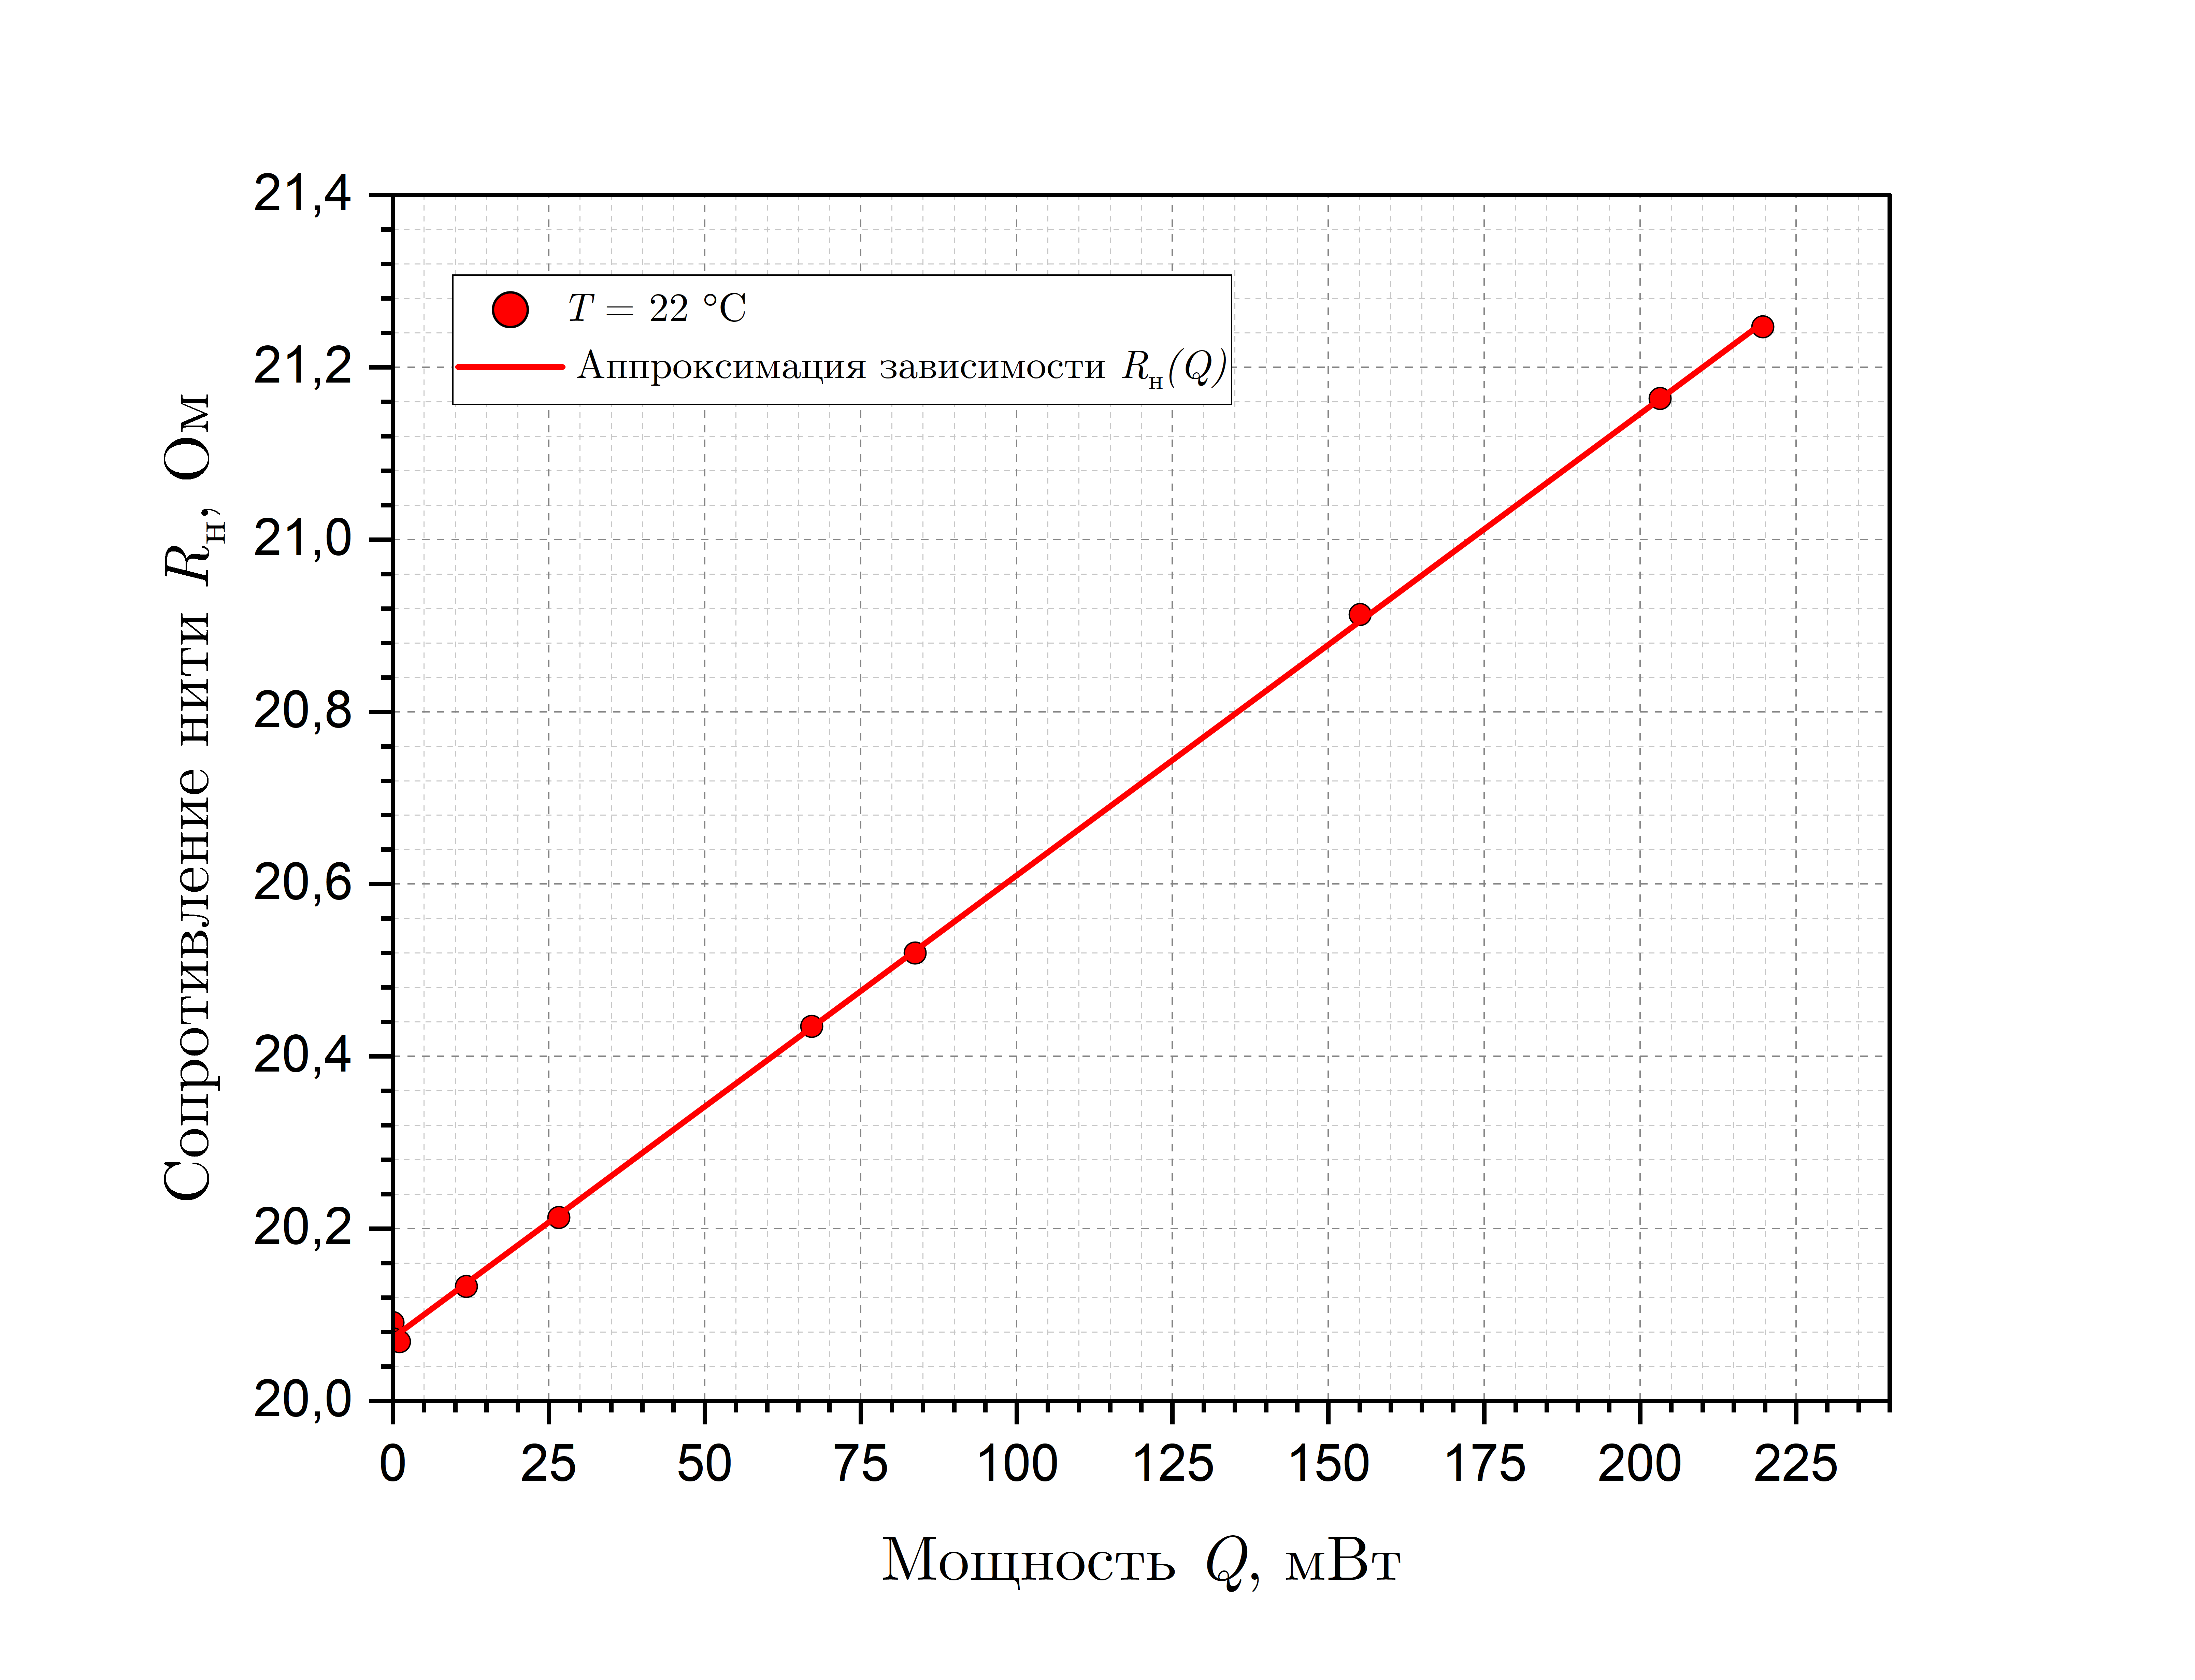
\includegraphics[width=0.8\textwidth]{images/R(Q)_22.png}
            \caption{График зависимости $R_{\text{н}}(Q)$ при $T = 22 ^\circ$C} 
            \label{graph:R(Q)_22}
        \end{figure}

        \begin{figure}[H]
            \centering
            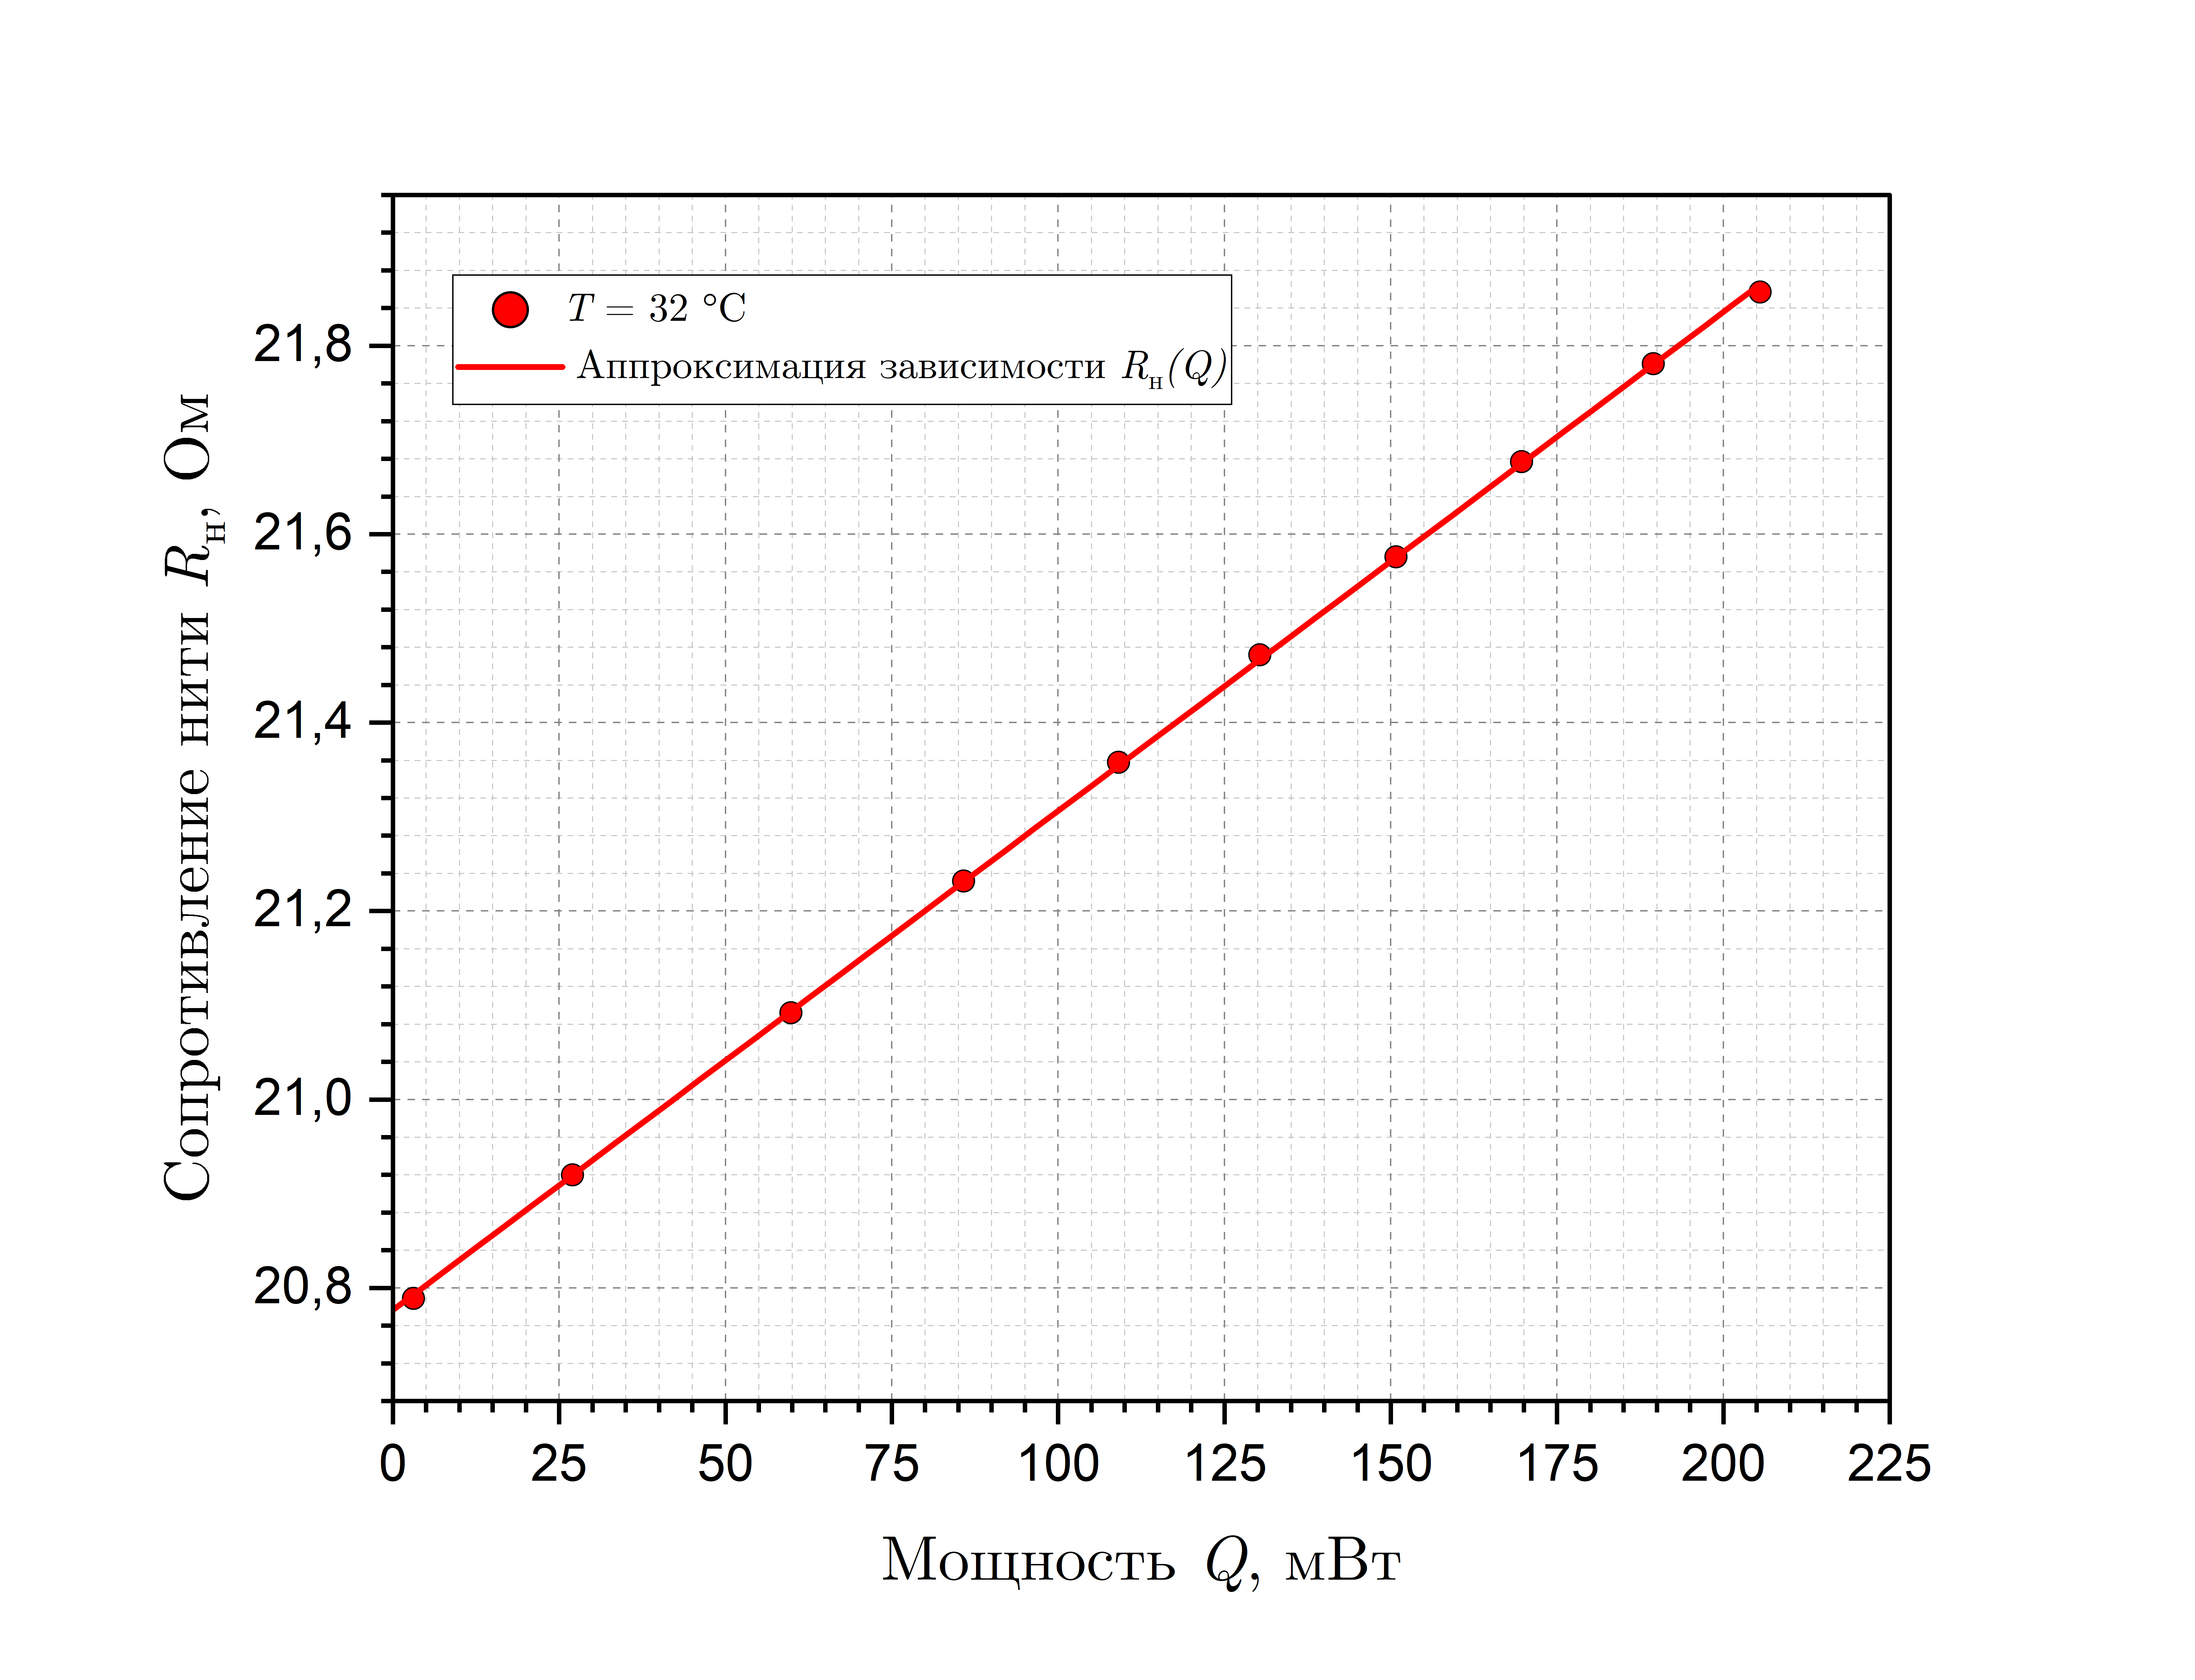
\includegraphics[width=0.8\textwidth]{images/R(Q)_32.png}
            \caption{График зависимости $R_{\text{н}}(Q)$ при $T = 32 ^\circ$C} 
            \label{graph:R(Q)_32}
        \end{figure}

        \begin{figure}[H]
            \centering
            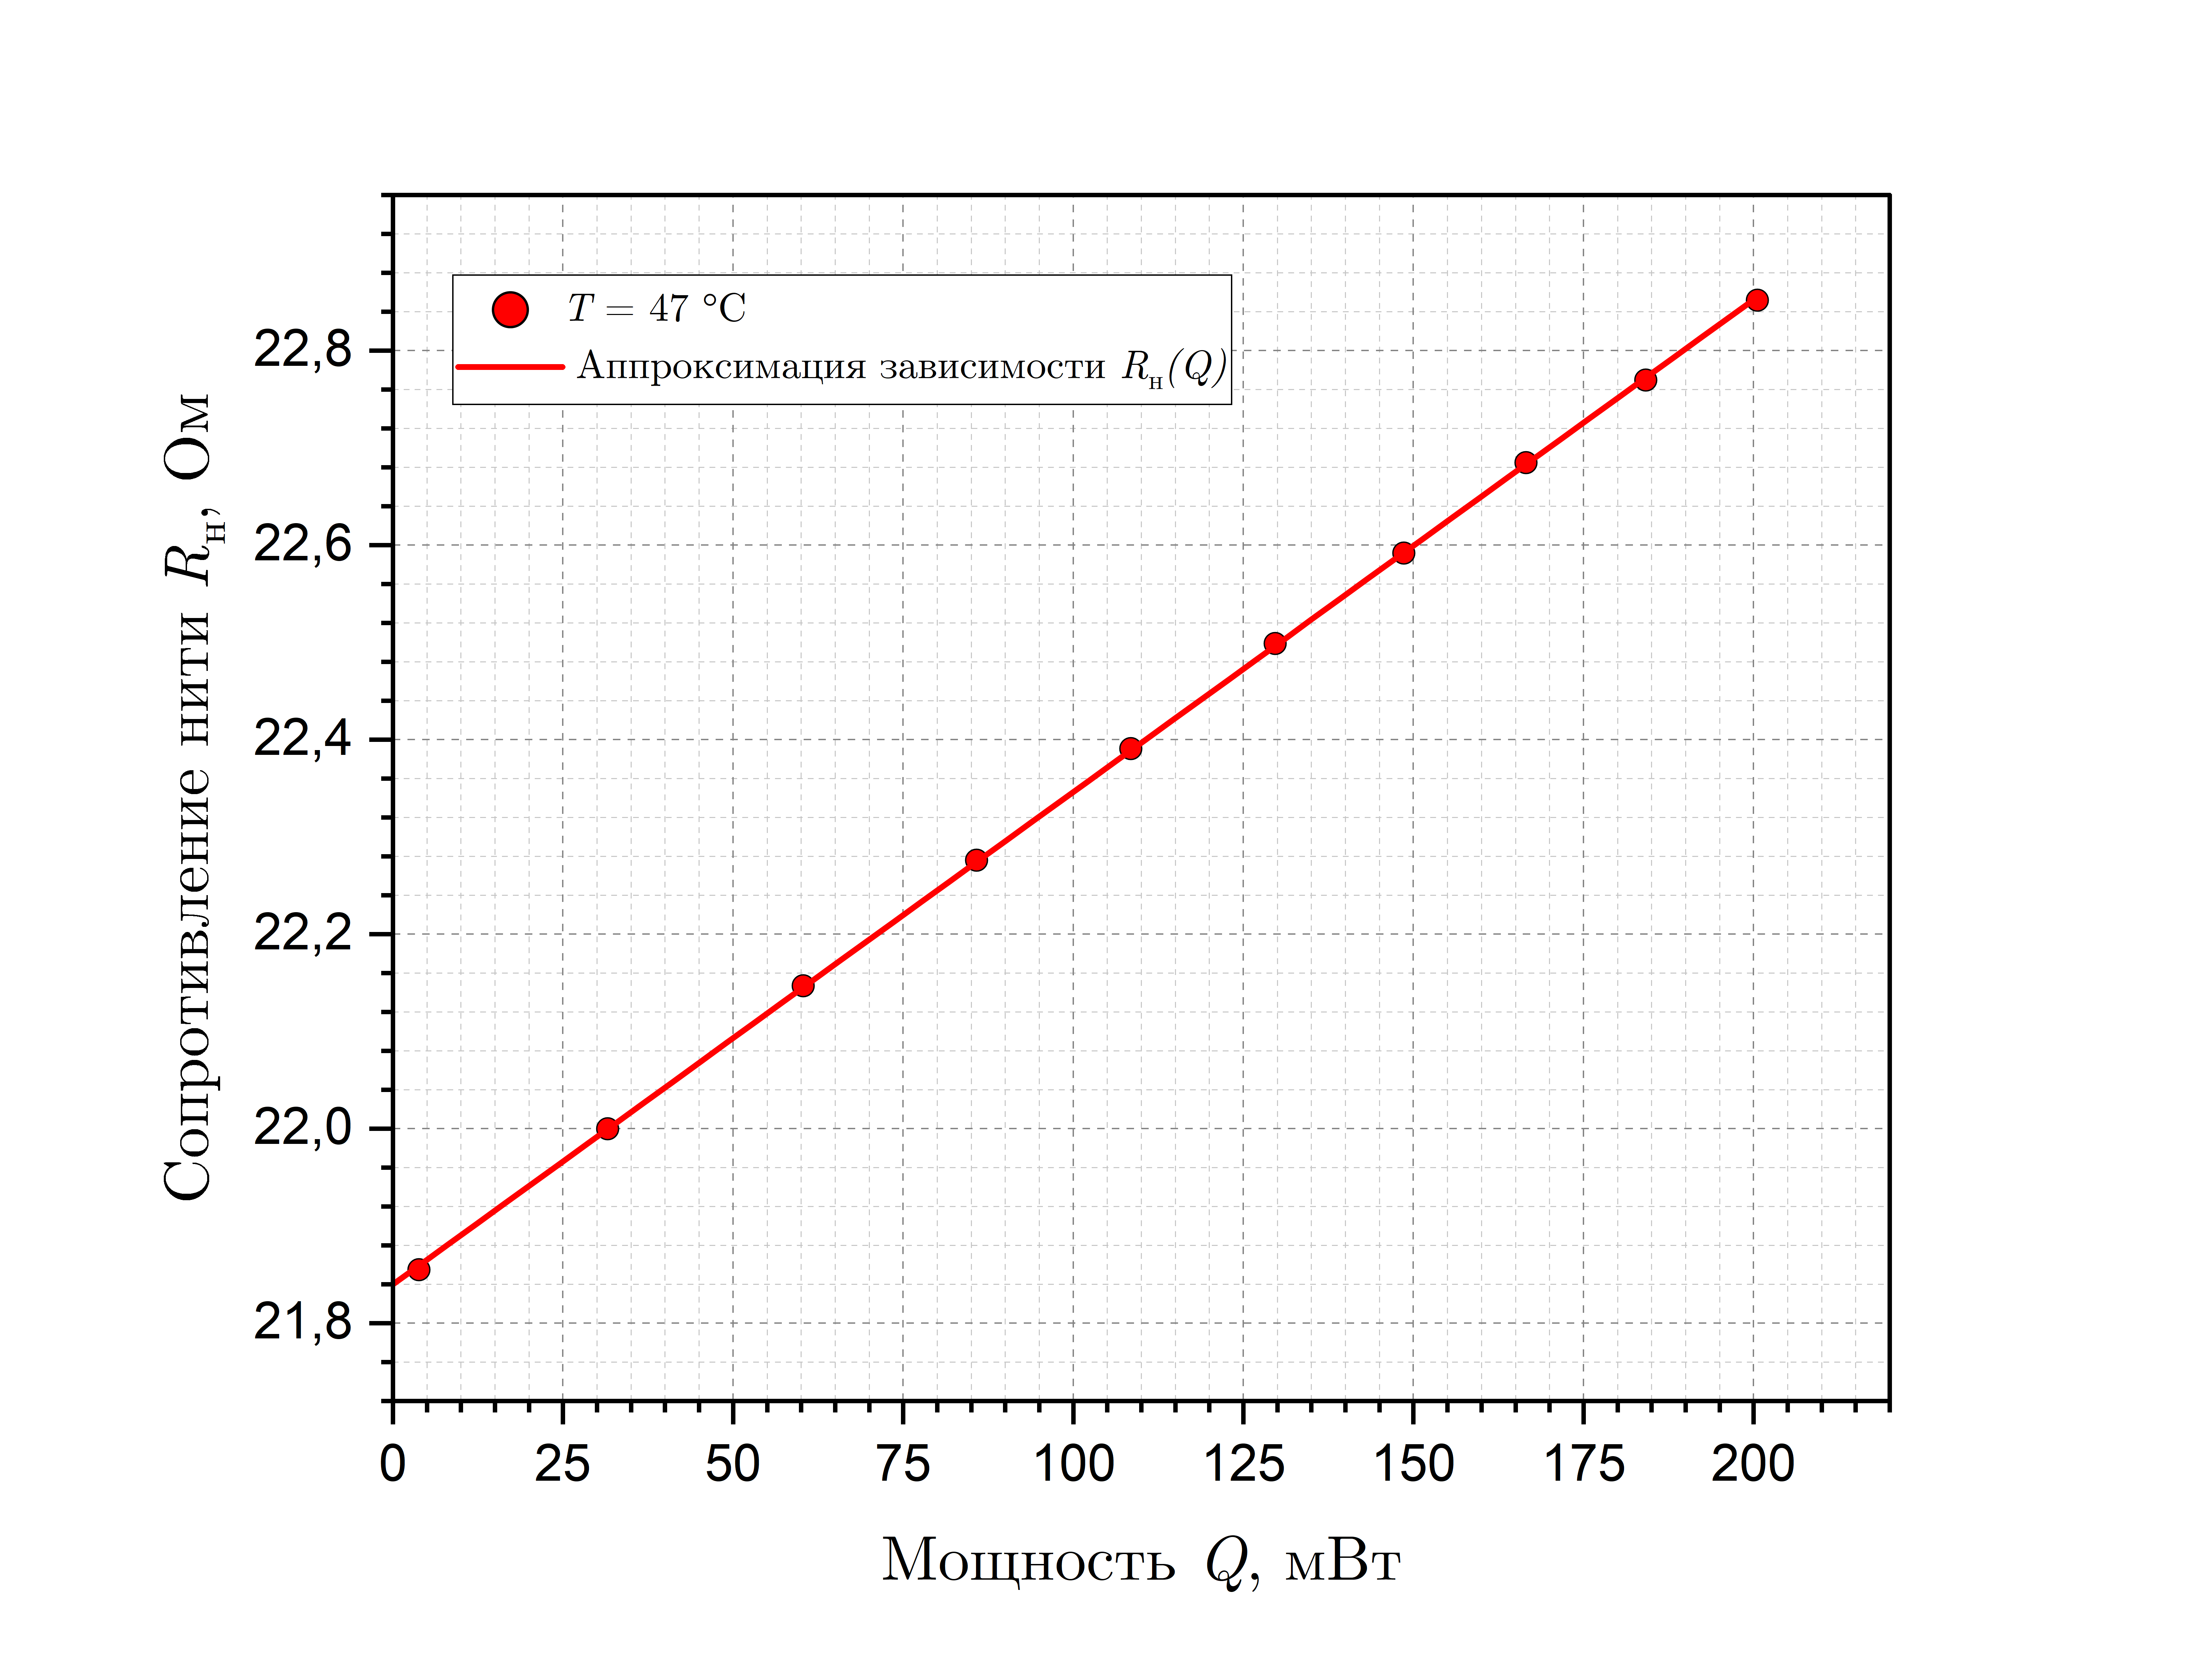
\includegraphics[width=0.8\textwidth]{images/R(Q)_47.png}
            \caption{График зависимости $R_{\text{н}}(Q)$ при $T = 47 ^\circ$C} 
            \label{graph:R(Q)_47}
        \end{figure}

        \begin{figure}[H]
            \centering
            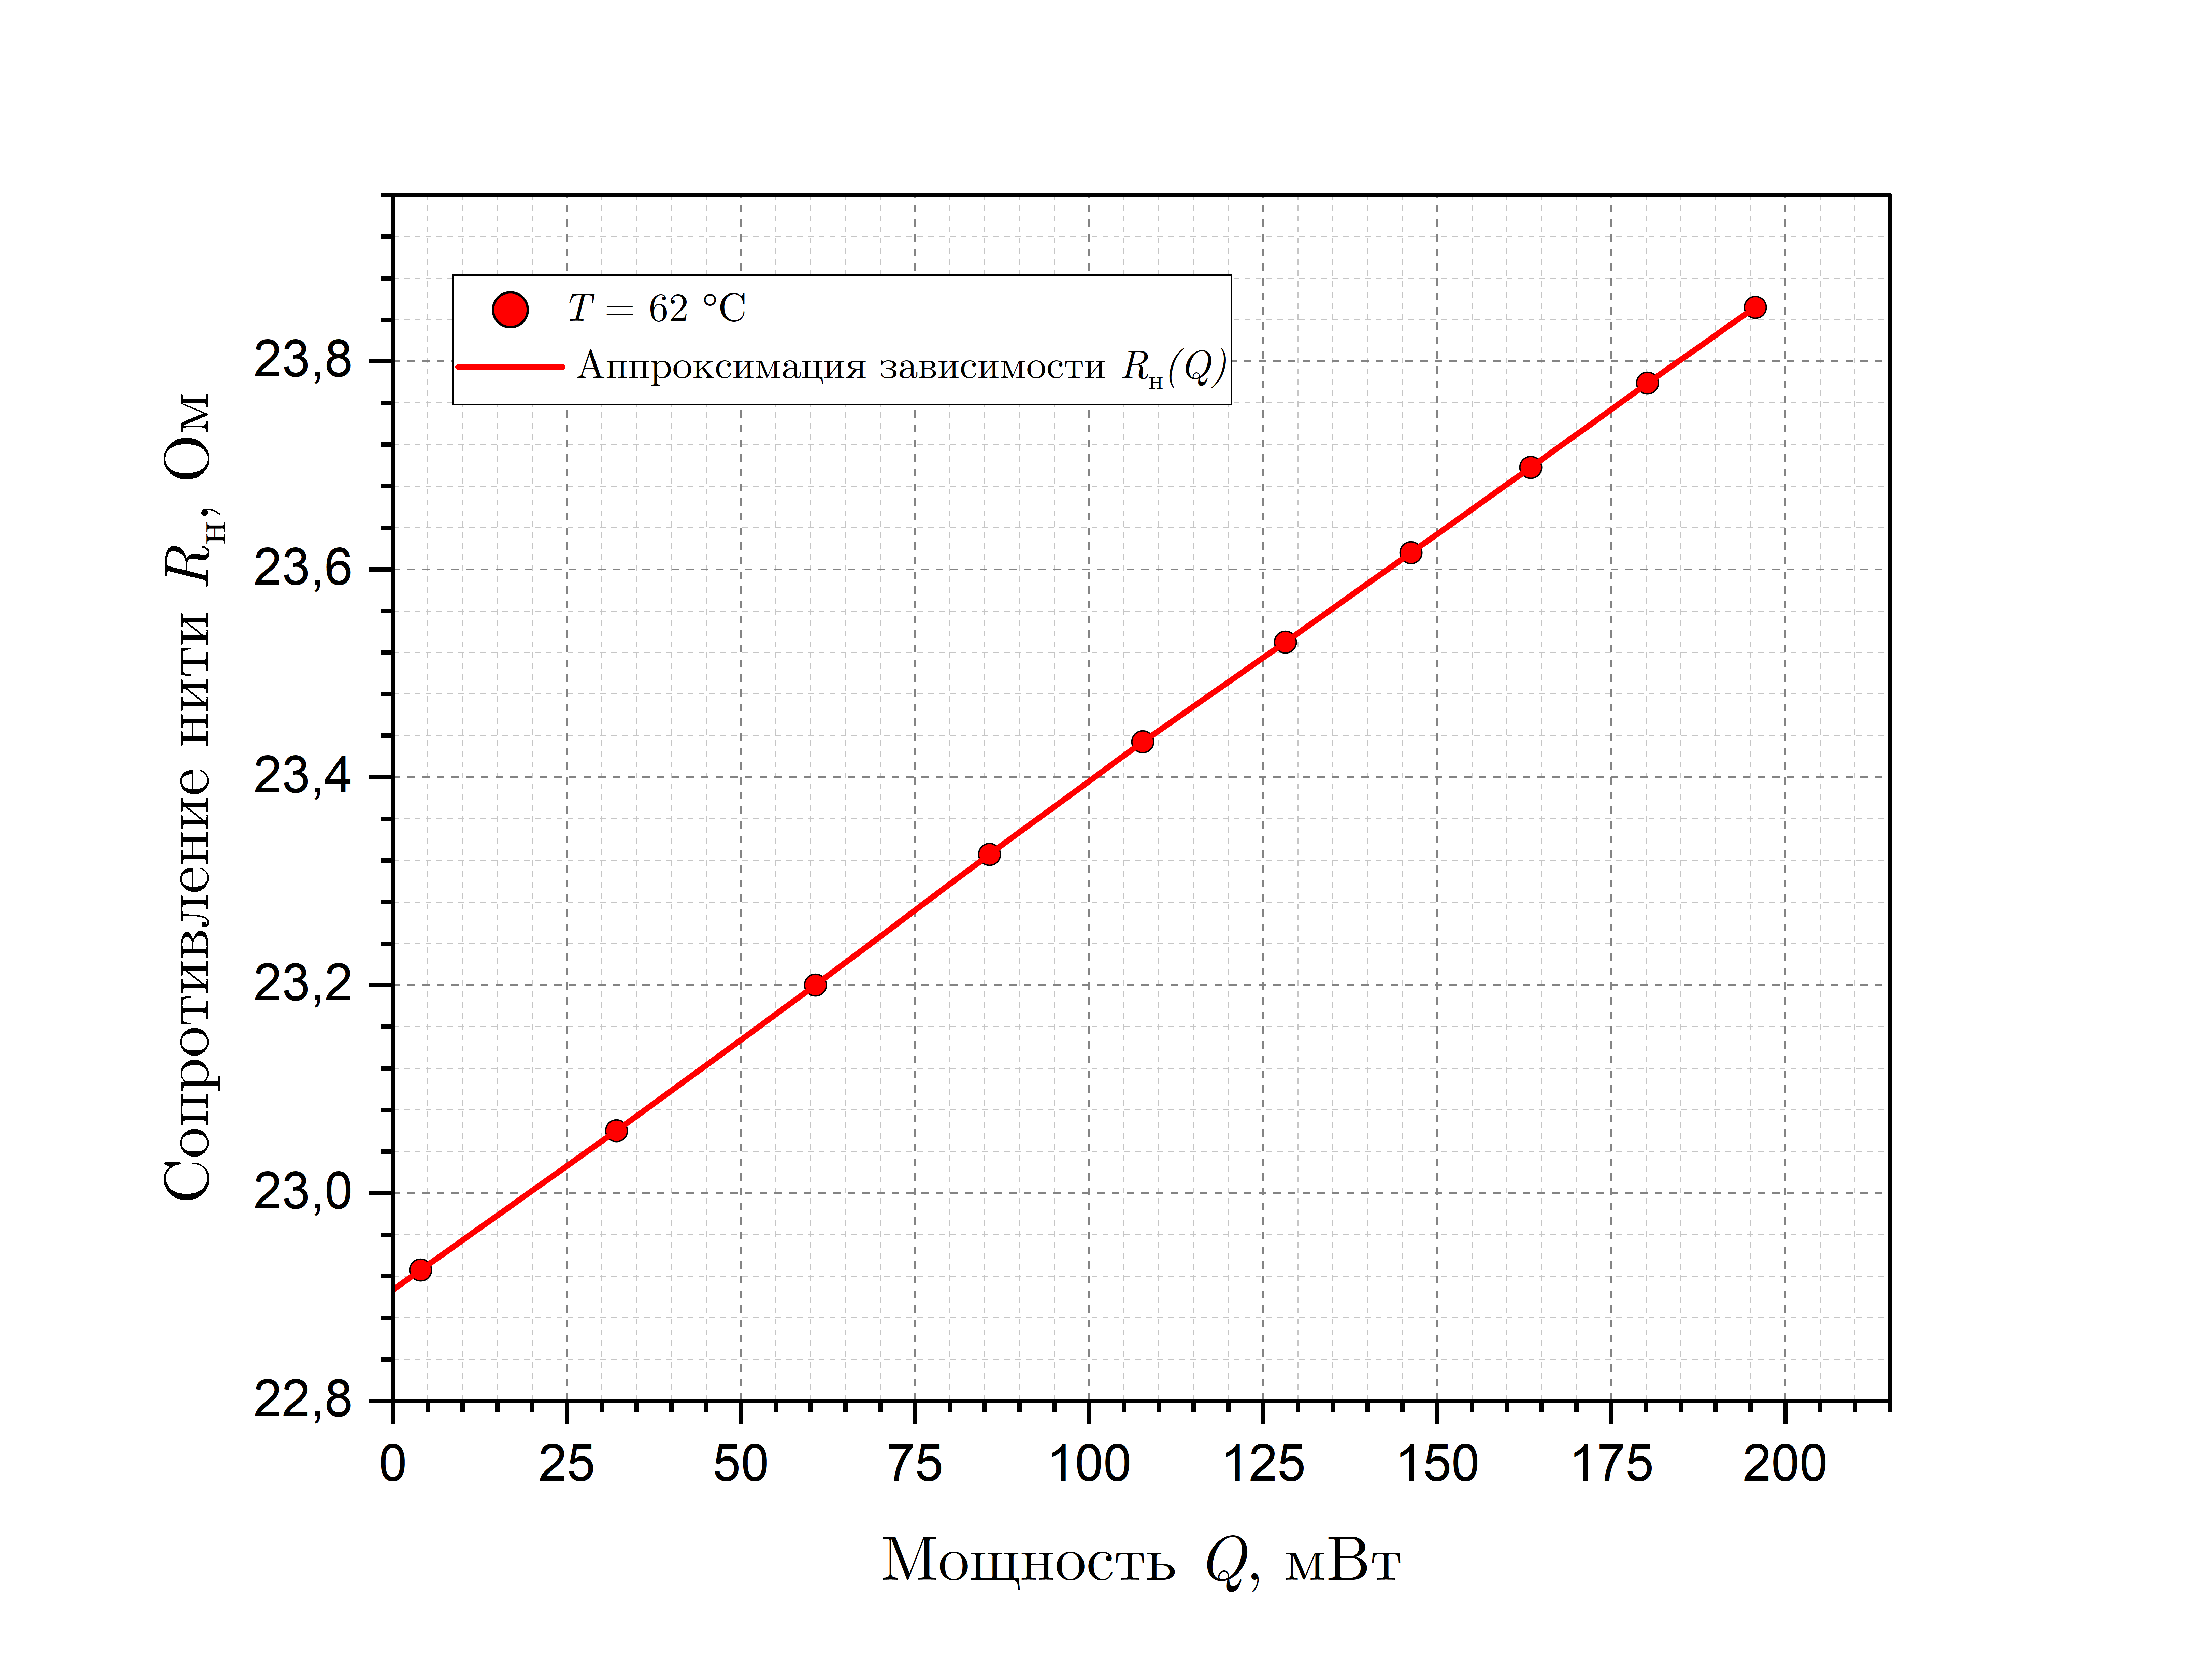
\includegraphics[width=0.8\textwidth]{images/R(Q)_62.png}
            \caption{График зависимости $R_{\text{н}}(Q)$ при $T = 62 ^\circ$C} 
            \label{graph:R(Q)_62}
        \end{figure}

        \begin{figure}[H]
            \centering
            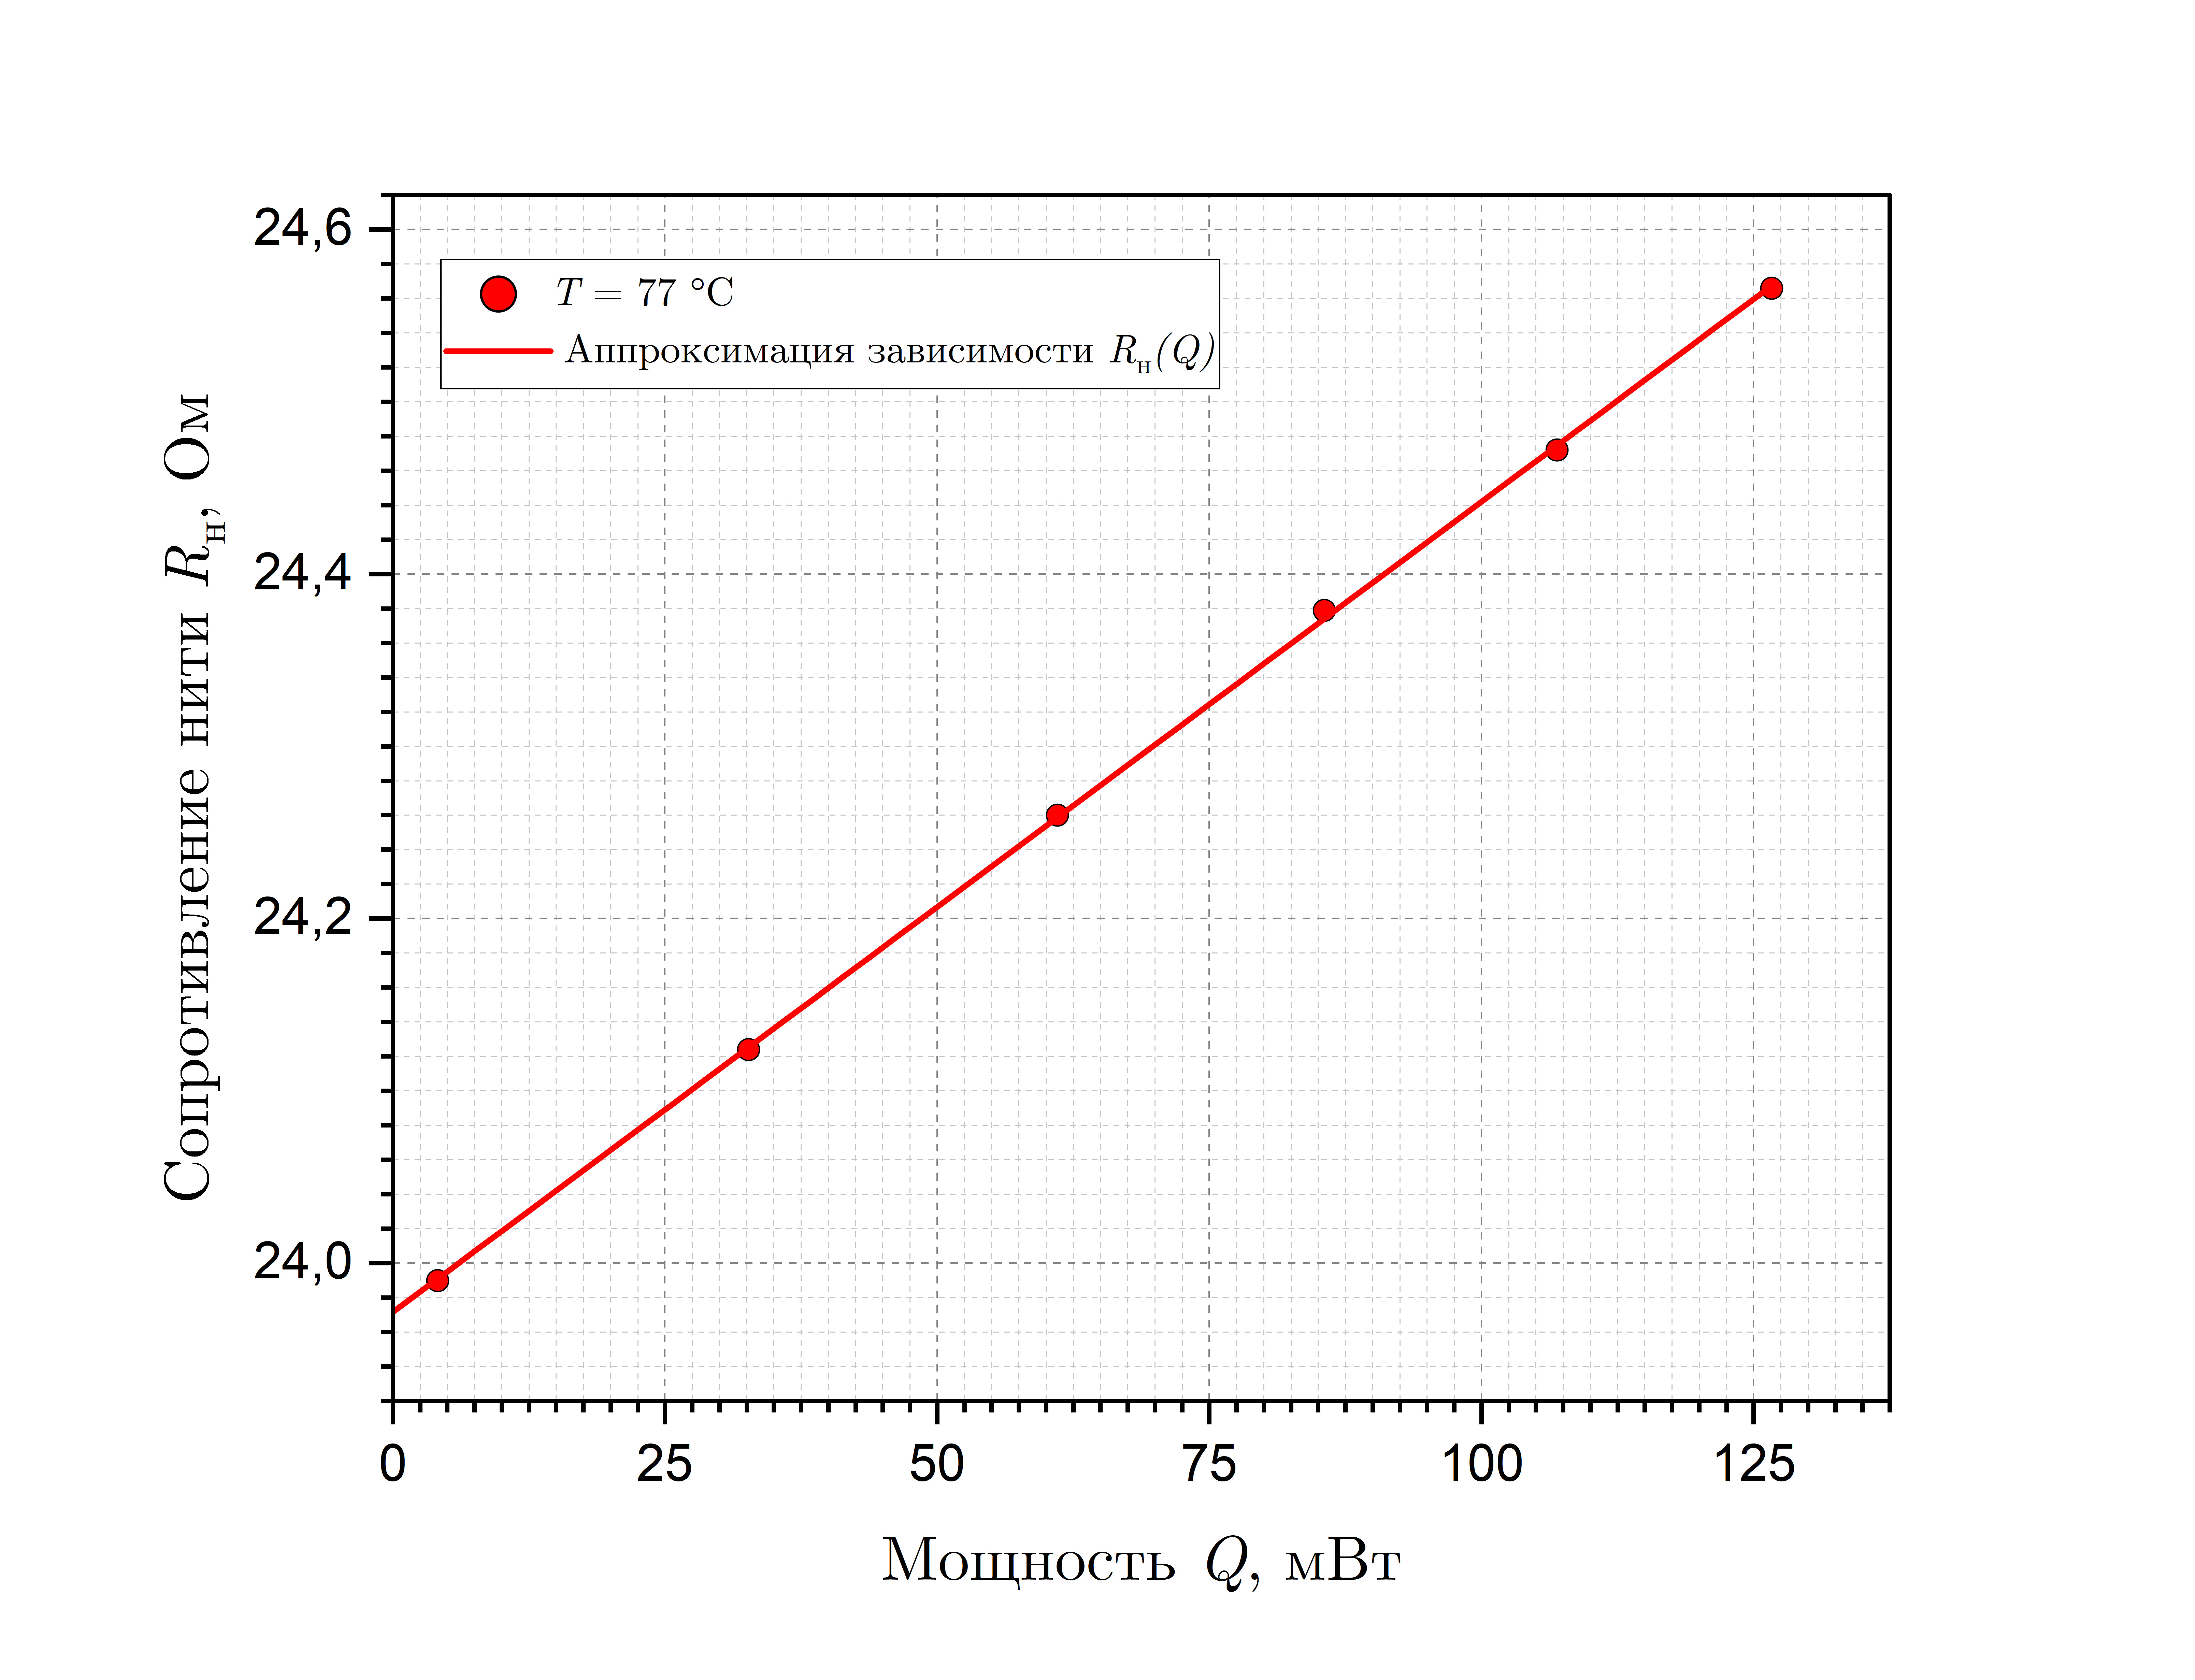
\includegraphics[width=0.8\textwidth]{images/R(Q)_77.png}
            \caption{График зависимости $R_{\text{н}}(Q)$ при $T = 77 ^\circ$C} 
            \label{graph:R(Q)_77}
        \end{figure}

        \begin{table}[H]
            \centering
            \begin{tabular}{|c|c|c|c|c|c|}
                \hline
                $T$, $^\circ$C            & 22,0   & 32,0   & 47,0   & 62,0   & 77,0  \\ \hline
                $R|_{Q = 0}$, Ом          & 20,073 & 20,777 & 21,840 & 22,908 & 23,972 \\ \hline
                $\sigma_{R|_{Q = 0}}$, Ом & 0,004  & 0,003  & 0,002  & 0,002  & 0,002 \\ \hline
                $dR/dQ$,          Ом/Вт   & 5,36   & 5,30   & 5,06   & 4,84   & 4,70 \\ \hline
                $\sigma_{dR/dQ}$, Ом/Вт   & 0,03   & 0,02   & 0,01   & 0,01   & 0,03 \\ \hline
            \end{tabular}
            \caption{Результаты вычислений.}
            \label{table:results_2}
        \end{table}

        \subsection*{Исследование зависимости $R(T)$. Определение температурного коэффициента сопротивления материала нити $\alpha$}
        
        \noindent Построим по значениям $R|_{Q = 0}$ график (рис.~\ref{graph:R(T)}) зависимости сопротивления нити от температуры $T$. Аппроксимацию прямой и расчет наклона $dR/dT$ произведем аналогично предыдущему пункту.
	
        \begin{figure}[H]
            \center{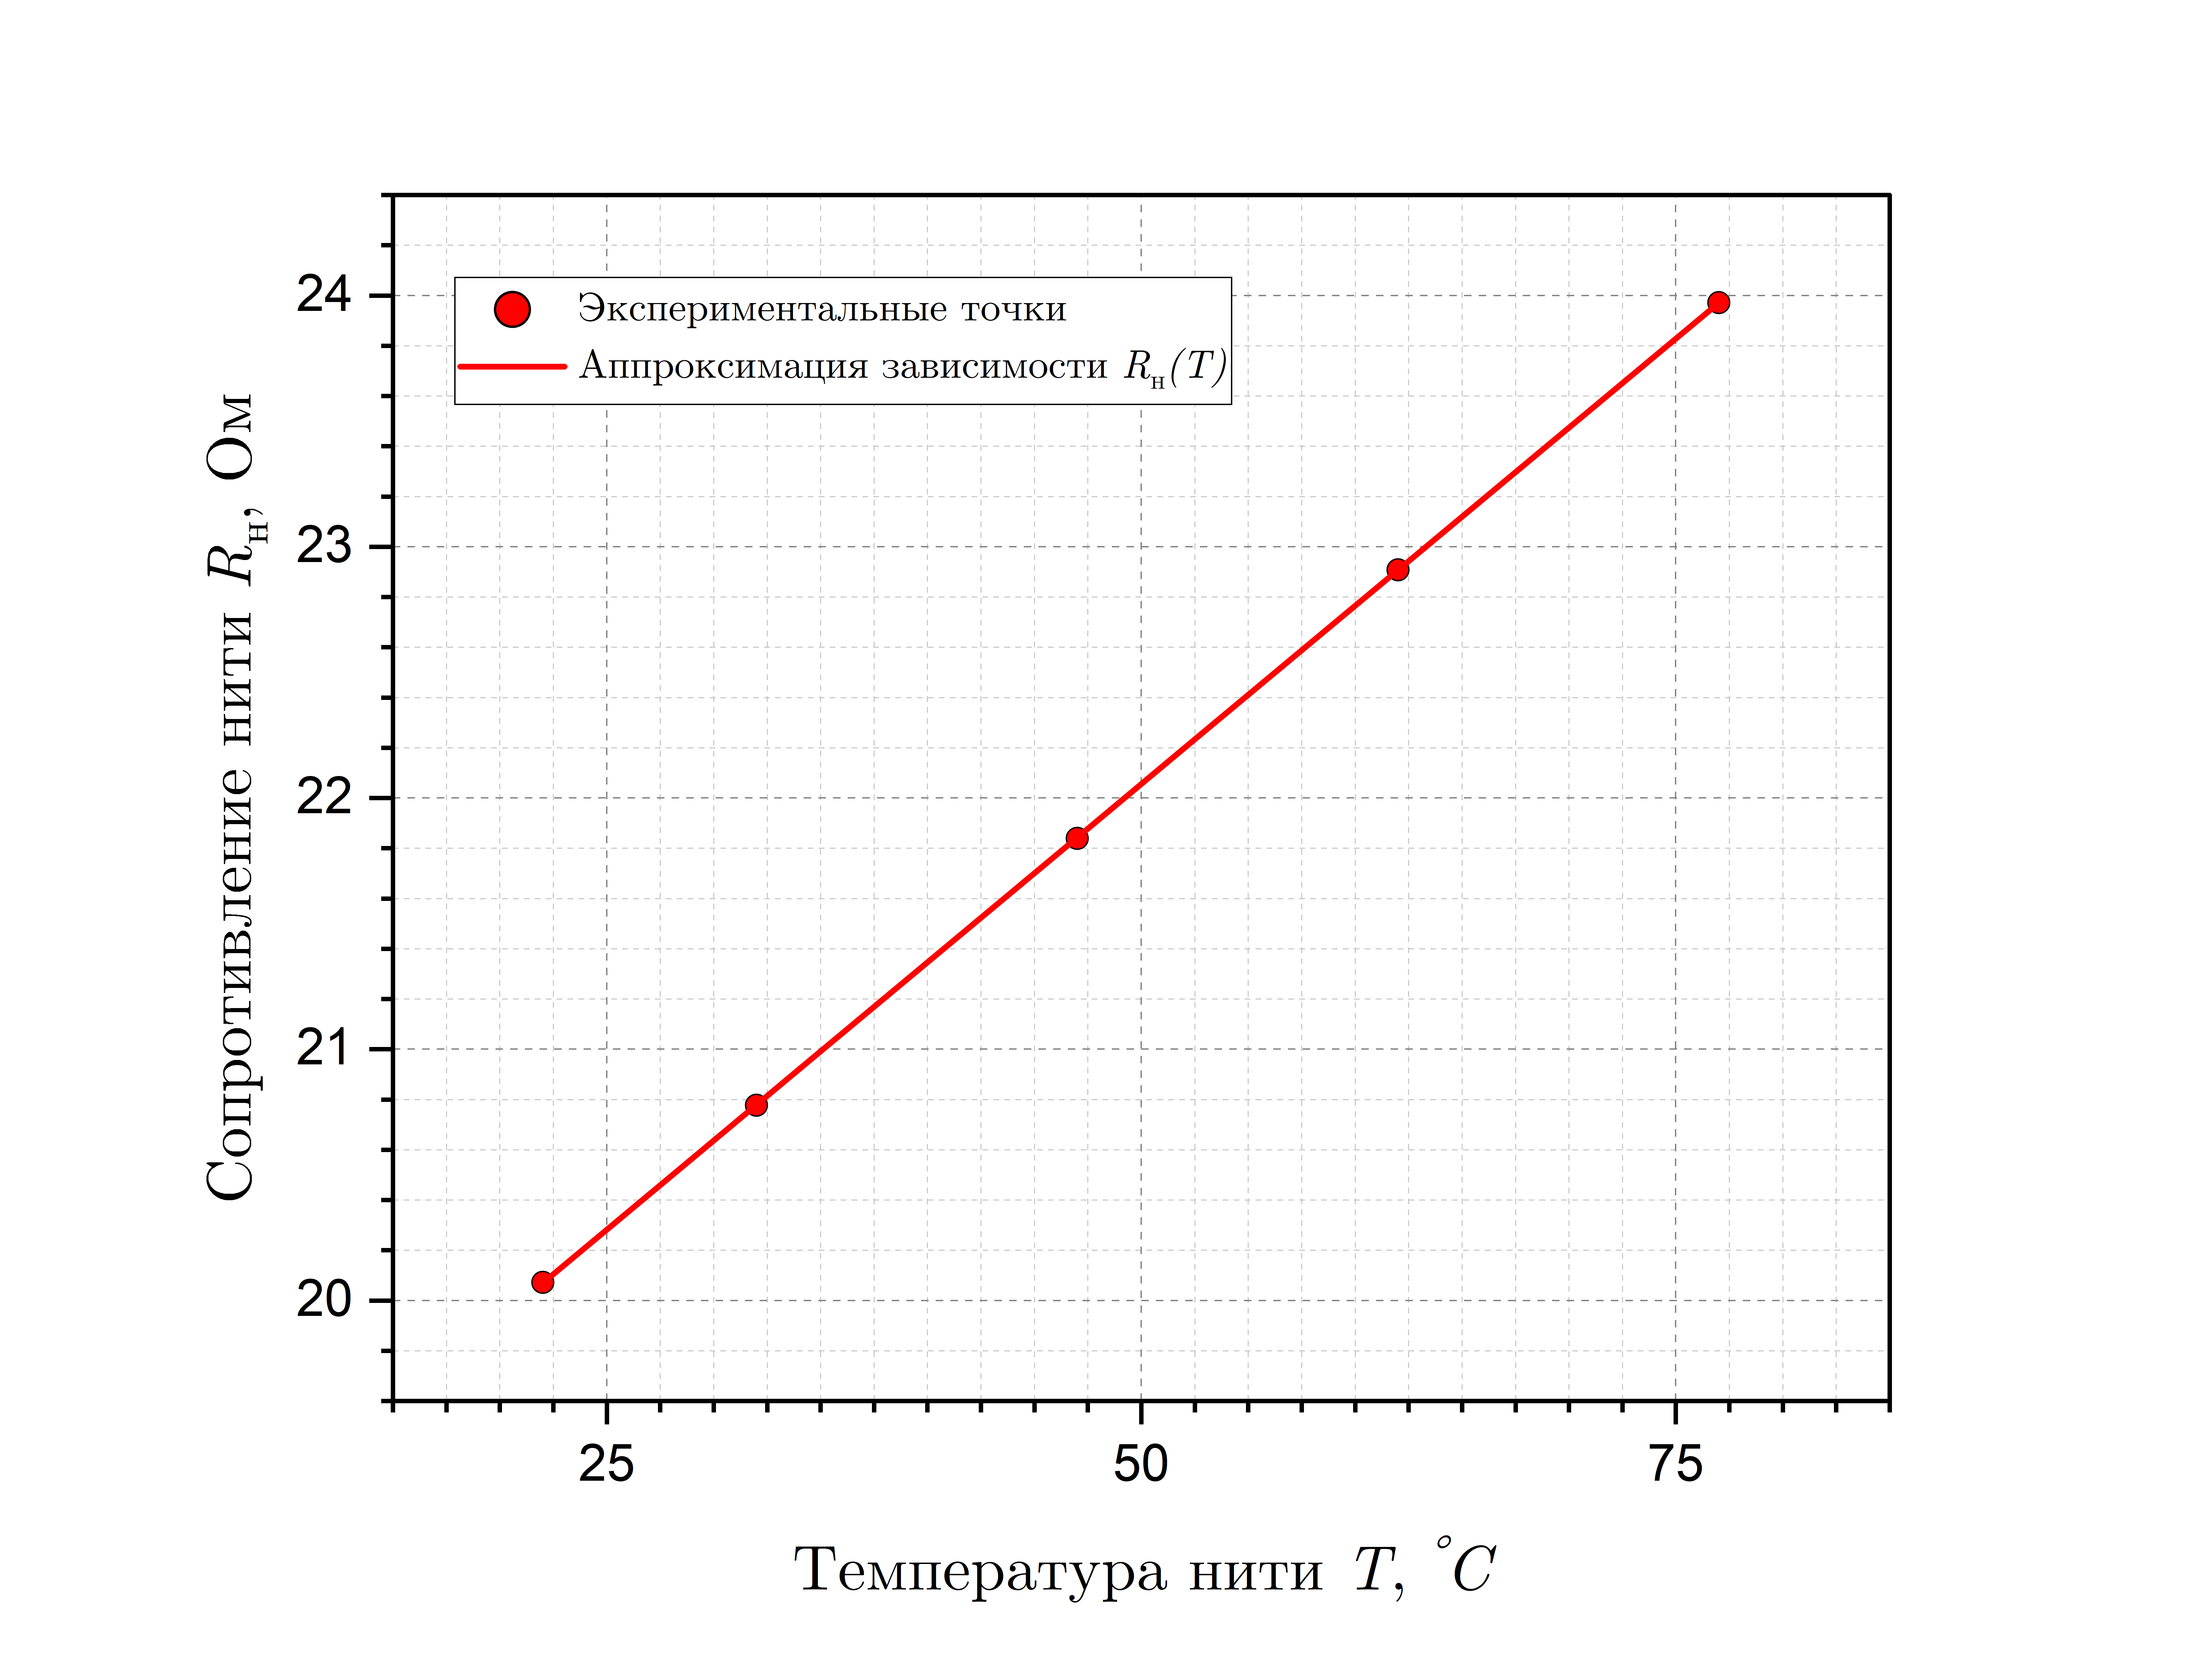
\includegraphics[width=0.8\textwidth]{images/R(T).png}}
            \caption{График зависимости $R = R(T)$}
            \label{graph:R(T)}
        \end{figure}

        \noindent Экспериментальные точки отлично ложатся на прямую, имеющую наклон: $dR/dT = \left(0,0709 \pm 0,0007 \right)$ Ом/К. \\

        \noindent Рассчитаем температурный коэффициент сопротивления материала нити $\alpha = \frac{1}{R_{273}} \frac{dR}{dT}$, где $R_{273} = 20$ Ом -- сопротивление платиновой нити при $0$ $^\circ$C. Получим, что температурный коэффициент сопротивления материала нити $\alpha = \left( 3,545 \pm 0,035\right) \cdot 10^{-3} \: K^{-1}$. Сравнивая это значение с табличным: $\alpha_{\text{табл}} = 3,8 \cdot 10^{3} \: K^{-1}$, замечаем, что полученный коэффициент равен табличному по порядку величины. 

        \subsection*{Определение экспериментальной зависимости $\kappa (T)$}

        \noindent Для каждой температуры прибора определим значение коэффициента теплопроводности газа по формуле $\kappa = \frac{dQ}{dR} \frac{dR}{dT} \frac{1}{2\pi L} \ln \frac{r_0}{r_1}$, где $2r_1 = \left(50 \pm 3 \right) \text{мкм}$, $2r_0 = \left(7,0 \pm 0,1 \right) \text{мм}$ и $L = \left(400 \pm 2 \right) \text{мм}$. \\
        
        \noindent Предполагая, что зависимость коэффициента теплопроводности от температуры имеет вид $\kappa = AT^\beta$, по полученным значениям построим аппроксимированную кривую рис.~\ref{graph:approxKappa}. Чтобы определить показатель степени $\beta$ построим график зависимости $\ln \kappa$ от $\ln T$. Результаты вычислений представлены в таблице~\ref{table:results_3}.
	
        \begin{table}[H]
            \centering
            \begin{tabular}{|c|ccccc|}
                \hline
                $T, K$ & \multicolumn{1}{c|}{295} & \multicolumn{1}{c|}{305} & \multicolumn{1}{c|}{320} & \multicolumn{1}{c|}{335} & 350 \\ \hline
                
                $dR/dQ, \text{Ом/Вт}$ & \multicolumn{1}{c|}{5,36} & \multicolumn{1}{c|}{5,3} & \multicolumn{1}{c|}{5,06} & \multicolumn{1}{c|}{4,84} & 4,7 \\ \hline
                
                $\sigma_{dR/dQ}, \text{Ом/Вт}$ & \multicolumn{1}{c|}{0,03} & \multicolumn{1}{c|}{0,02} & \multicolumn{1}{c|}{0,01} & \multicolumn{1}{c|}{0,01} & 0,03 \\ \hline
                
                $dQ/dR, \text{Вт/Ом}$ & \multicolumn{1}{c|}{0,1866} & \multicolumn{1}{c|}{0,1887} & \multicolumn{1}{c|}{0,1976} & \multicolumn{1}{c|}{0,2066} & 0,2128 \\ \hline
                
                $\sigma_{dQ/dR}, \text{Вт/Ом}$ & \multicolumn{1}{c|}{0,0010} & \multicolumn{1}{c|}{0,0007} & \multicolumn{1}{c|}{0,0004} & \multicolumn{1}{c|}{0,0004} & 0,0014 \\ \hline
                
                $dR/dT, \text{Ом/К}$ & \multicolumn{5}{c|}{0,0709} \\ \hline
                $\sigma_{dR/dT}, \text{Ом/К}$ & \multicolumn{5}{c|}{0,0007} \\ \hline
                
                $\kappa, \text{Вт/(К} \cdot \text{м)}$ & \multicolumn{1}{c|}{26,0} & \multicolumn{1}{c|}{26,3} & \multicolumn{1}{c|}{27,6} & \multicolumn{1}{c|}{28,8} & 29,7 \\ \hline
                
                $\sigma_\kappa, \text{Вт/(К} \cdot \text{м)}$ & \multicolumn{1}{c|}{1,0} & \multicolumn{1}{c|}{1,1} & \multicolumn{1}{c|}{1,1} & \multicolumn{1}{c|}{1,2} & 1,2 \\ \hline
                
                $\ln \kappa$ & \multicolumn{1}{c|}{3,26}   & \multicolumn{1}{c|}{3,27}   & \multicolumn{1}{c|}{3,32}   & \multicolumn{1}{c|}{3,36}   & 3,39   \\ \hline
                
                $\sigma_{\ln \kappa}$ & \multicolumn{1}{c|}{0,04} & \multicolumn{1}{c|}{0,04} & \multicolumn{1}{c|}{0,04} & \multicolumn{1}{c|}{0,04} & 0,04 \\ \hline
                
                $\ln T$ & \multicolumn{1}{c|}{5,6870} & \multicolumn{1}{c|}{5,7203} & \multicolumn{1}{c|}{5,7683} & \multicolumn{1}{c|}{5,8141} & 5,8579 \\ \hline
            \end{tabular}
            \caption{Результаты вычислений коэффициентов теплопроводности газа $\kappa$ для каждой температуры термостата $T_0$}
            \label{table:results_3}
        \end{table}

        \begin{figure}[H]
            \centering
            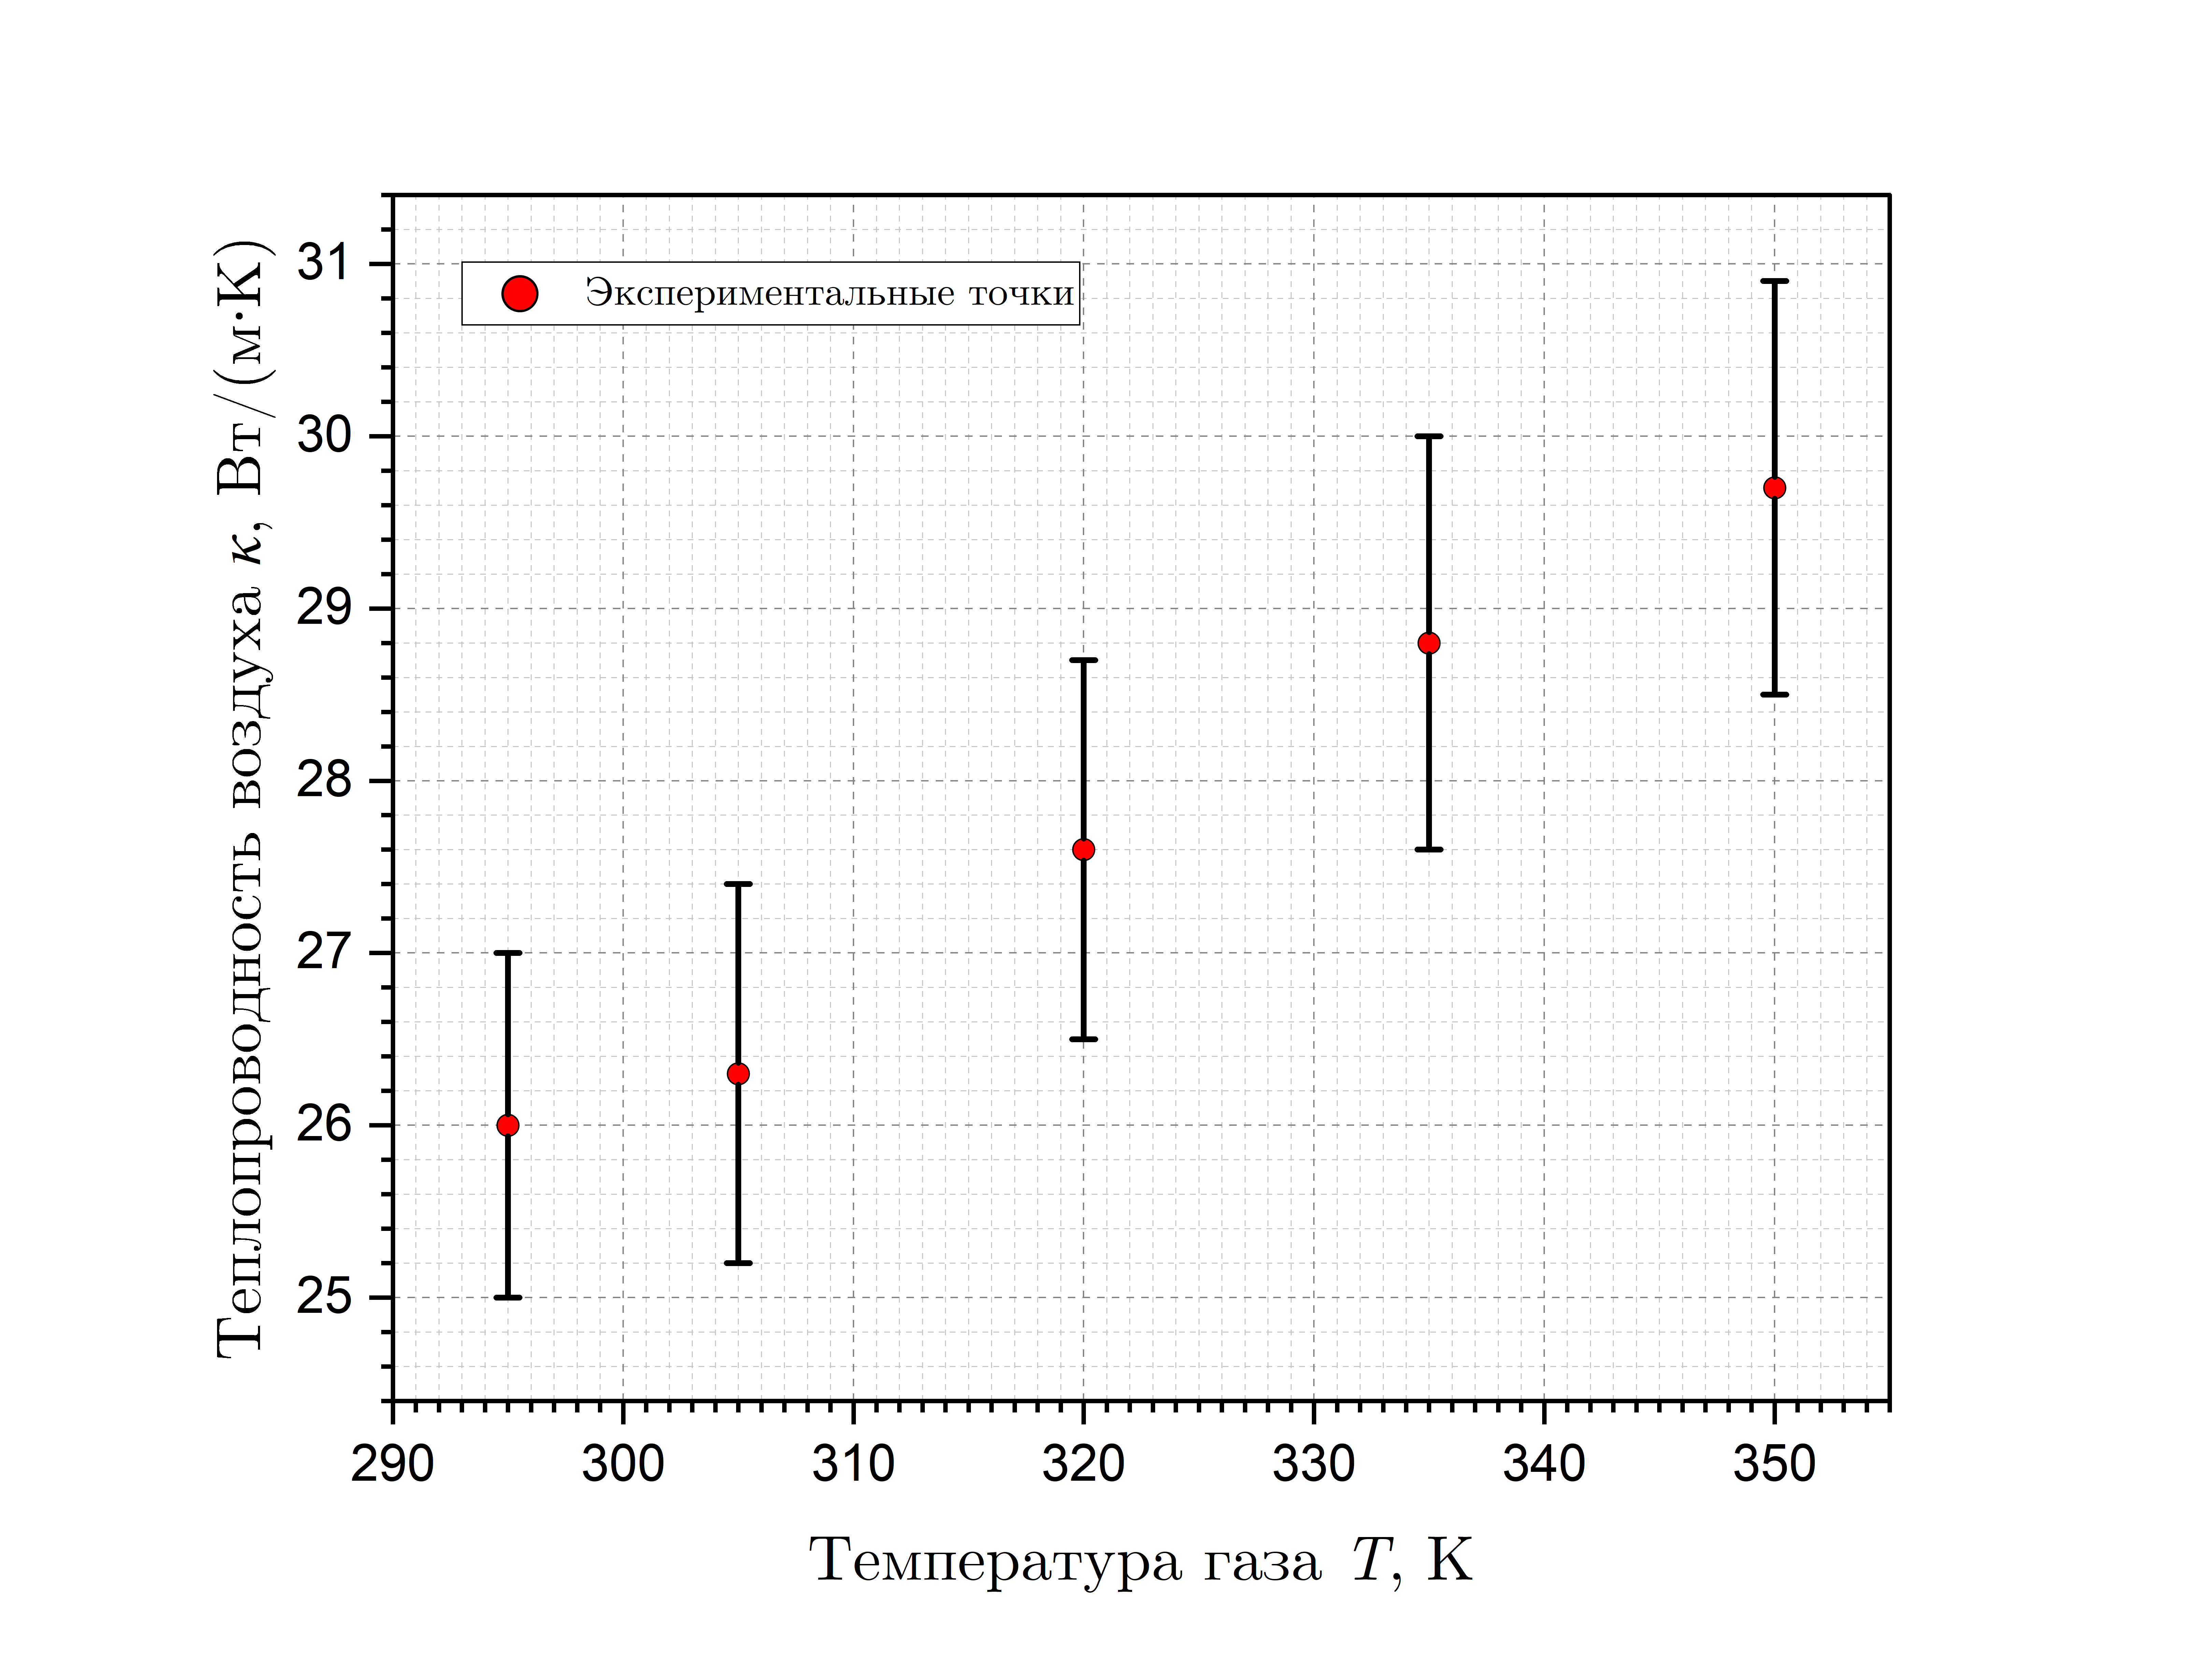
\includegraphics[width=0.8\textwidth]{images/Kappa(T).png}
            \caption{График зависимости $\kappa (T)$} 
            \label{graph:kappa}
        \end{figure}

        \begin{figure}[H]
            \centering
            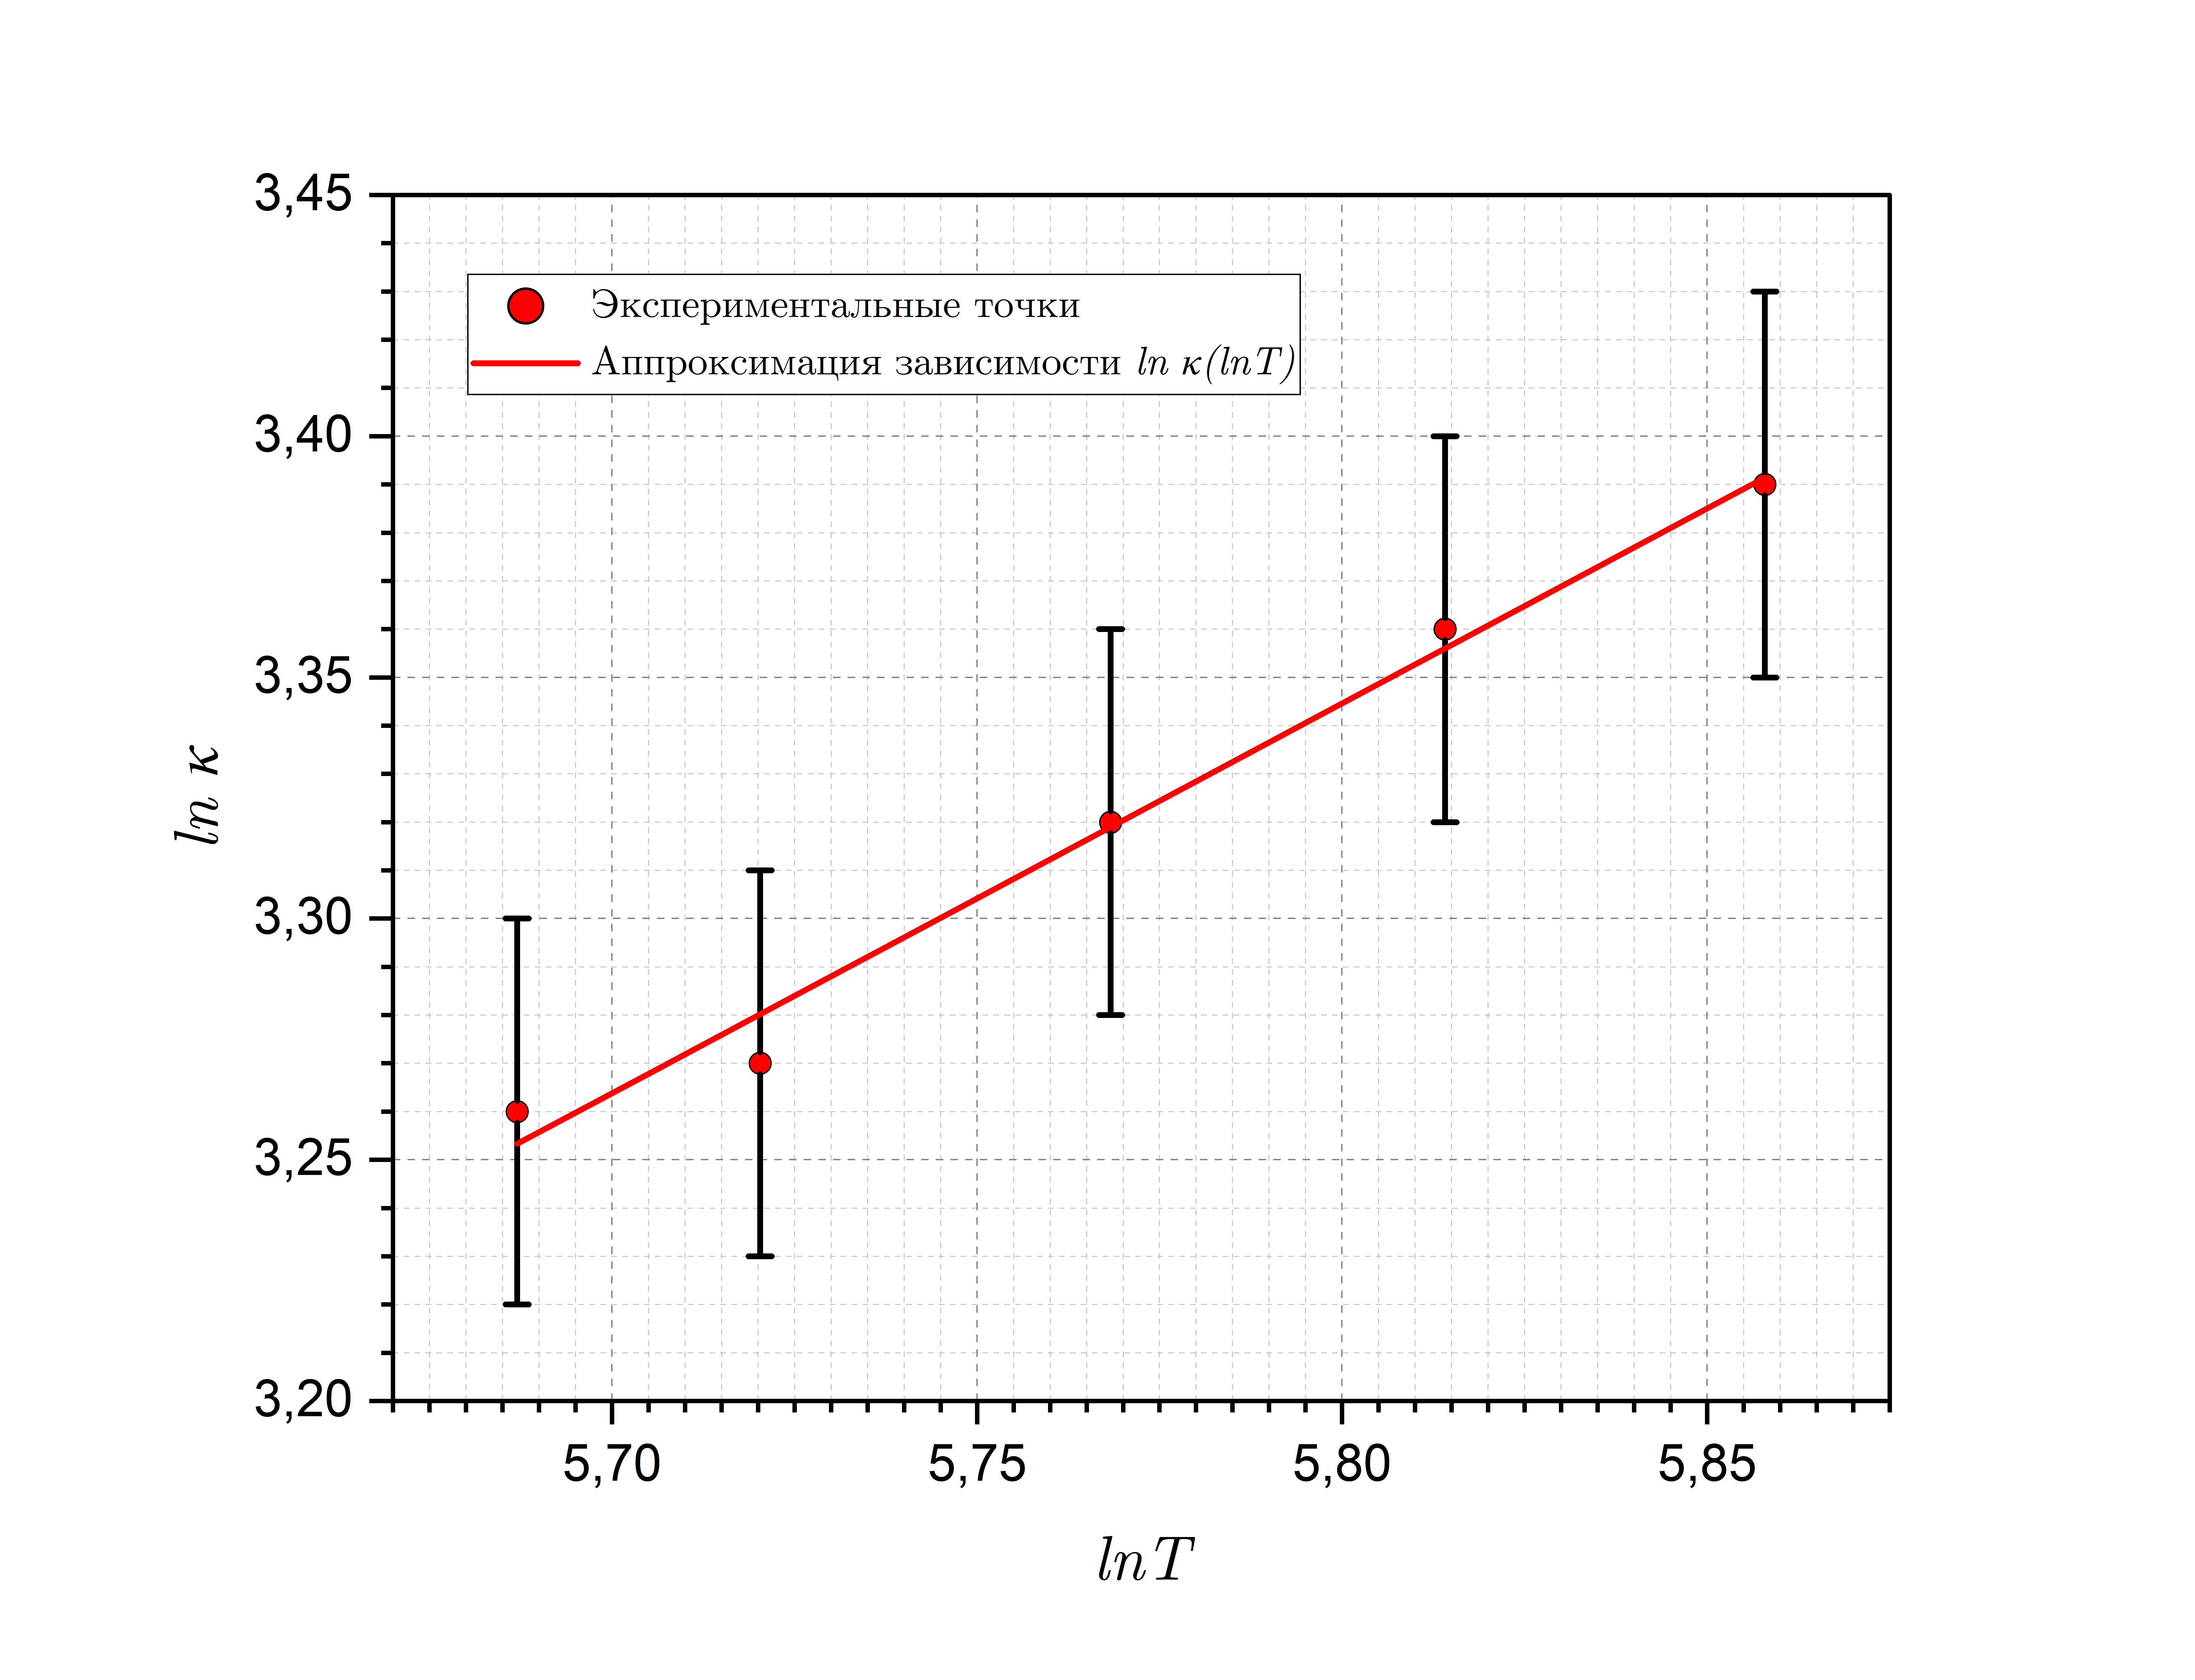
\includegraphics[width=0.8\textwidth]{images/lnK(lnT).png}
            \caption{График зависимости $\ln \kappa (\ln T)$} 
            \label{graph:approxKappa}
        \end{figure}

        \noindent Аппроксимацию прямой (рис.~\ref{graph:approxKappa}) произведем методом наименьших квадратов в компьютерной программе \textit{Origin Pro 2023}. Имеем: $\beta = \left(0,81 \pm 0,05\right)$.

    \section*{Заключение}
        
        \noindent В ходе данной работы мы определили коэффициент теплопроводности воздуха при атмосферном давлении и разных температурах по теплоотдаче нагреваемой током нити в цилиндрическом сосуде. В среднем каждое значение коэффициента теплопроводности отличается от табличного при данной температуре не более, чем на 5\%. По полученным результатам рассчитали коэффициент $\beta$ в формуле $\kappa = AT^\beta$: $\beta = \left(0,81 \pm 0,05\right)$. Однако полученный результат с учетом погрешности не соотвествует теоретическому значению $\beta = 0,5$ ($\kappa \propto \sqrt{T}$), то есть наш результат завышен на 62\%. Удивительно, что если построить аналогичным образом прямую, используя табличные значения коэффициента теплопроводности воздуха при атмосферном давлении, то $\beta = 0,81$, что сходится с полученным значением. Разница в результатах, во-первых, может быть связана с неучтенными тепловыми потерями через основания цилиндра. Во-вторых, при выводе формулы (\ref{formula}) не учитывалась зависимость теплопроводности от температуры (поэтому она справедлива только при $\Delta T \ll T$) и молекулы воздуха рассматривались, как одинаковые \textit{твердые шарики}. И наконец, возникновение термо-ЭДС (эффект Зеебека) повлияло на точность вольтметра.\\

        \noindent Также был определён температурный коэффициент сопротивления материала нити $\alpha = \left( 3,545 \pm 0,035\right) \cdot 10^{-3} \: K^{-1}$, что сходится с табличным $\alpha_{\text{табл}} = 3,8 \cdot 10^{3} \: K^{-1}$ по порядку величины.

\end{document}